\documentclass[aspectratio=169, 11pt]{beamer}

% ── Theme & Colors ──────────────────────────────────────────
\usetheme{Madrid}
\usecolortheme{default}

% Custom color palette
\definecolor{deepblue}{RGB}{20, 66, 114}
\definecolor{accentblue}{RGB}{41, 128, 185}
\definecolor{lightblue}{RGB}{214, 234, 248}
\definecolor{accentorange}{RGB}{230, 126, 34}
\definecolor{accentgreen}{RGB}{39, 174, 96}
\definecolor{darkgray}{RGB}{52, 73, 94}
\definecolor{lightgray}{RGB}{236, 240, 241}
\definecolor{accentred}{RGB}{192, 57, 43}
\definecolor{softpurple}{RGB}{142, 68, 173}

\setbeamercolor{structure}{fg=deepblue}
\setbeamercolor{palette primary}{bg=deepblue, fg=white}
\setbeamercolor{palette secondary}{bg=accentblue, fg=white}
\setbeamercolor{palette tertiary}{bg=deepblue!80, fg=white}
\setbeamercolor{frametitle}{bg=deepblue, fg=white}
\setbeamercolor{title}{fg=white}
\setbeamercolor{subtitle}{fg=lightblue}
\setbeamercolor{block title}{bg=accentblue, fg=white}
\setbeamercolor{block body}{bg=lightblue!30}
\setbeamercolor{block title alerted}{bg=accentorange, fg=white}
\setbeamercolor{block body alerted}{bg=accentorange!10}
\setbeamercolor{block title example}{bg=accentgreen, fg=white}
\setbeamercolor{block body example}{bg=accentgreen!10}
\setbeamercolor{item}{fg=accentblue}

% Remove navigation symbols
\setbeamertemplate{navigation symbols}{}

% Slide numbers
\setbeamertemplate{footline}{%
  \hfill\insertframenumber/\inserttotalframenumber\hspace*{4pt}\vspace{2pt}%
}

% ── Packages ────────────────────────────────────────────────
\usepackage{tikz}
\usetikzlibrary{shapes.geometric, arrows.meta, positioning, calc, fit, backgrounds, decorations.pathreplacing}
% fontawesome5 not available on this system — using text symbols instead
\newcommand{\faRobot}{\ensuremath{\diamond}}
\newcommand{\faMortarPestle}{\ensuremath{\triangleright}}
\newcommand{\faDatabase}{\ensuremath{\boxdot}}
\newcommand{\faBook}{\ensuremath{\triangleleft}}
\newcommand{\faBrain}{\ensuremath{\star}}
\newcommand{\faCubes}{\ensuremath{\square}}
\newcommand{\faFlask}{\ensuremath{\circ}}
\newcommand{\faSync}{\ensuremath{\circlearrowleft}}
\newcommand{\faKeyboard}{\ensuremath{\Rightarrow}}
\newcommand{\faFileAlt}{\ensuremath{\boxminus}}
\newcommand{\faTable}{\ensuremath{\equiv}}
\newcommand{\faCube}{\ensuremath{\square}}
\usepackage{booktabs}
\usepackage{graphicx}
\usepackage{colortbl}
\usepackage{adjustbox}

% ── Metadata ────────────────────────────────────────────────
\title{Enzyme Discovery Agent}
\subtitle{An LLM-Driven Autonomous Workflow}
\author{R. Zhu}
\date{\today}

\begin{document}

% ════════════════════════════════════════════════════════════
% SLIDE 1: Title
% ════════════════════════════════════════════════════════════
{
\setbeamercolor{background canvas}{bg=deepblue}
\begin{frame}[plain]
\vfill
\begin{center}
{\Huge\bfseries\color{white} Enzyme Discovery Agent}\\[12pt]
{\Large\color{lightblue} An LLM-Driven Autonomous Workflow\\for Biocatalyst Identification}\\[24pt]
{\large\color{white} R. Zhu}\\[6pt]
{\normalsize\color{lightblue!70} \today}
\end{center}
\vfill
\end{frame}
}

% ════════════════════════════════════════════════════════════
% SLIDE 2: Motivation — Problem + Application Context
% ════════════════════════════════════════════════════════════
\begin{frame}{Why an Enzyme Discovery Agent?}
\begin{columns}[T]
\begin{column}{0.48\textwidth}
\begin{alertblock}{The Challenge}
\begin{itemize}
\item Enzyme discovery requires searching \textbf{multiple databases} (UniProt, KEGG, InterPro, PubMed)
\item Relevant enzymes scattered across \textbf{diverse EC classes}
\item Manual search misses enzymes with \textbf{incomplete annotations}
\item Biochemical \textbf{reasoning} needed to evaluate candidates
\end{itemize}
\end{alertblock}
\end{column}
\begin{column}{0.48\textwidth}
\begin{exampleblock}{Our Solution}
\begin{itemize}
\item \textbf{Autonomous LLM agent} orchestrates search and evaluation
\item \textbf{18 specialized tools} across 6 categories
\item Structured \textbf{reasoning framework} with persistent notebook
\item \textbf{Dual-ranked reports}: confidence vs.\ suitability
\end{itemize}
\end{exampleblock}
\end{column}
\end{columns}

\vspace{4pt}
\begin{center}
\colorbox{lightblue!50}{\parbox{0.88\textwidth}{\centering
\small\textbf{Key principle:} No hardcoded enzyme names or pathways --- all discovery emerges from LLM reasoning + tool execution.
}}
\end{center}
\end{frame}

% ════════════════════════════════════════════════════════════
% SLIDE 2b: Design Philosophy
% ════════════════════════════════════════════════════════════
\begin{frame}{Design Philosophy}
\vspace{-8pt}
\begin{columns}[T]
\begin{column}{0.48\textwidth}

\begin{alertblock}{\small No Composite Scoring}
\vspace{-2pt}
\begin{itemize}\scriptsize
\setlength\itemsep{1pt}
\item \texttt{evaluate\_candidate()} returns \textbf{raw data only}: UniProt metadata, EC match depth, substrate similarity, paper counts, structural availability
\item No numeric score --- the LLM applies \textbf{biochemistry reasoning} to rank
\item Rationale: composite weights are brittle and domain-dependent; a 0.4 Tanimoto with correct mechanism may outrank 0.8 with wrong bond direction
\end{itemize}
\end{alertblock}

\begin{block}{\small Principle-Driven, Not Phase-Rigid}
\vspace{-2pt}
\begin{itemize}\scriptsize
\setlength\itemsep{1pt}
\item 7 principles (P1--P7) embedded in system prompt guide behavior
\item Agent infers its own phase from iteration count + candidate count
\item Can backtrack: if discovery yields 0 hits, broaden search before advancing
\item Phases are a \textit{recommended} workflow, not a state machine
\end{itemize}
\end{block}

\end{column}
\begin{column}{0.48\textwidth}

\begin{exampleblock}{\small Structured Validation via Hard \& Soft Gates}
\vspace{-2pt}
\begin{itemize}\scriptsize
\setlength\itemsep{1pt}
\item \textbf{Hard gates} (critical warnings): bond-type mismatch, direction mismatch, severe size mismatch --- require specific PMID to override
\item \textbf{Soft gates} (weaknesses): moderate size mismatch, low characterization, TrEMBL status --- LLM can weigh contextually
\item \textbf{Substrate classification}: polymer, carrier-tethered, peptide vs.\ amide --- prevents cross-class false positives
\end{itemize}
\end{exampleblock}

\vspace{2pt}
\begin{center}
\colorbox{lightblue!50}{\parbox{0.92\textwidth}{\centering
\scriptsize\textbf{Key insight:} The evaluator provides \textit{structured facts} (bond types, FG counts, MW ratios). The LLM provides \textit{biochemical judgment} (which facts matter for this specific target). Hard gates prevent the LLM from overriding thermodynamic constraints.
}}
\end{center}

\end{column}
\end{columns}
\end{frame}

% ════════════════════════════════════════════════════════════
% SLIDE 3: System Architecture + 4 Phases (combined)
% ════════════════════════════════════════════════════════════
\begin{frame}{System Architecture}
\begin{center}
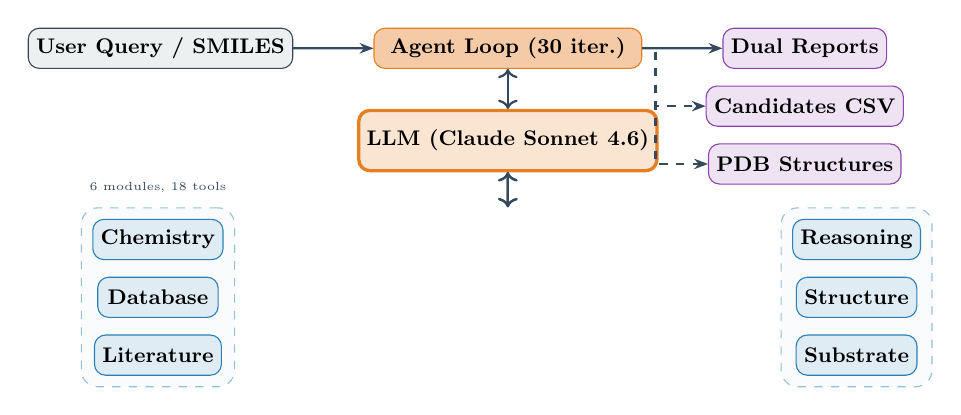
\begin{tikzpicture}[
    scale=0.85, transform shape,
    node distance=0.5cm and 0.6cm,
    every node/.style={font=\small},
    box/.style={rectangle, rounded corners=4pt, minimum width=2.0cm, minimum height=0.6cm, text centered, font=\small\bfseries},
    llmbox/.style={box, fill=accentorange!20, draw=accentorange, line width=1.2pt, minimum width=3.0cm, minimum height=0.9cm},
    toolbox/.style={box, fill=accentblue!15, draw=accentblue, minimum width=1.8cm},
    outbox/.style={box, fill=softpurple!15, draw=softpurple, minimum width=2.0cm},
    arr/.style={-{Stealth[length=5pt]}, thick, color=darkgray},
    darr/.style={-{Stealth[length=5pt]}, thick, color=darkgray, dashed},
]

% LLM Core
\node[llmbox] (llm) {LLM (Claude Sonnet 4.6)};

% Tool categories (left side)
\node[toolbox, below left=0.7cm and 2.0cm of llm] (chem) {Chemistry};
\node[toolbox, below=0.25cm of chem] (db) {Database};
\node[toolbox, below=0.25cm of db] (lit) {Literature};

% Tool categories (right side)
\node[toolbox, below right=0.7cm and 2.0cm of llm] (reason) {Reasoning};
\node[toolbox, below=0.25cm of reason] (struct) {Structure};
\node[toolbox, below=0.25cm of struct] (sub) {Substrate};

% Agent Loop
\node[box, fill=accentorange!40, draw=accentorange, above=0.6cm of llm, minimum width=4.0cm] (agent) {Agent Loop (30 iter.)};

% Input
\node[box, fill=lightgray, draw=darkgray, left=1.2cm of agent, minimum width=2.2cm] (input) {User Query / SMILES};

% Outputs
\node[outbox, right=1.2cm of agent] (report) {Dual Reports};
\node[outbox, below=0.25cm of report] (csv) {Candidates CSV};
\node[outbox, below=0.25cm of csv] (structs) {PDB Structures};

% Tool group fit
\begin{scope}[on background layer]
\node[fit=(chem)(db)(lit), draw=accentblue!50, dashed, rounded corners=6pt, inner sep=4pt, fill=accentblue!3] (leftfit) {};
\node[fit=(reason)(struct)(sub), draw=accentblue!50, dashed, rounded corners=6pt, inner sep=4pt, fill=accentblue!3] (rightfit) {};
\end{scope}

% Arrows
\draw[arr] (input) -- (agent);
\draw[arr] (agent) -- (report);
\draw[arr, <->] (agent) -- (llm);
\draw[arr, <->] (llm) -- (leftfit.north-|llm);
\draw[arr, <->] (llm) -- (rightfit.north-|llm);
\draw[darr] (agent.east) -- ++(0.2,0) |- (csv.west);
\draw[darr] (agent.east) -- ++(0.2,0) |- (structs.west);

% Labels
\node[font=\tiny\color{darkgray}, above=0.1cm of leftfit] {6 modules, 18 tools};

\end{tikzpicture}
\end{center}
\end{frame}

% ════════════════════════════════════════════════════════════
% SLIDE 4: 4-Phase Discovery Workflow
% ════════════════════════════════════════════════════════════
\begin{frame}{Discovery Workflow --- 4 Phases}
\begin{center}
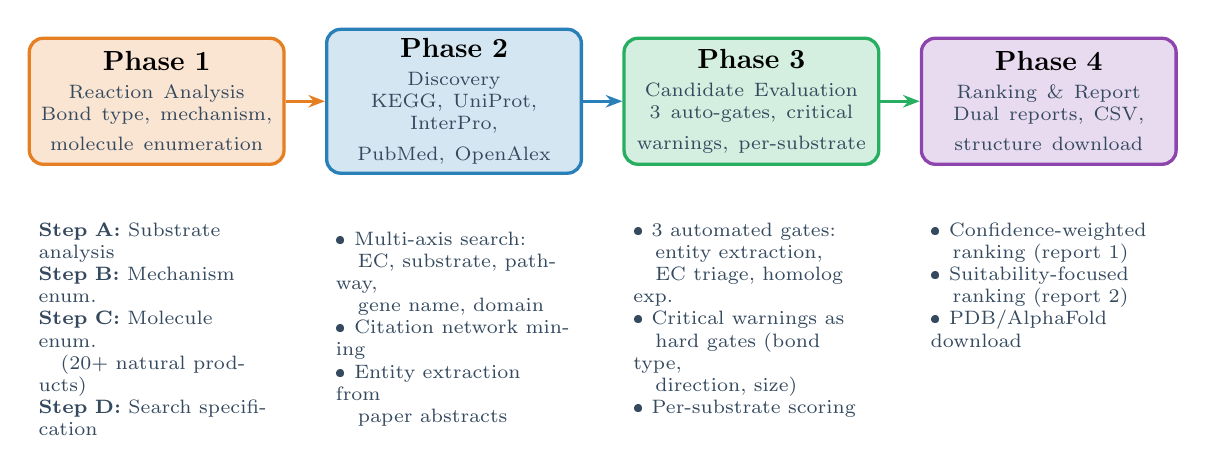
\begin{tikzpicture}[
    node distance=0.2cm,
    phase/.style={rectangle, rounded corners=5pt, minimum width=3.2cm, minimum height=1.6cm, text centered, font=\small\bfseries, text width=3.0cm},
    arr/.style={-{Stealth[length=6pt]}, very thick},
]

% Phase boxes
\node[phase, fill=accentorange!20, draw=accentorange, line width=1.2pt] (p1) {
\normalsize Phase 1\\[2pt]
\scriptsize\normalfont\color{darkgray}
Reaction Analysis\\
Bond type, mechanism,\\
molecule enumeration
};

\node[phase, fill=accentblue!20, draw=accentblue, line width=1.2pt, right=0.5cm of p1] (p2) {
\normalsize Phase 2\\[2pt]
\scriptsize\normalfont\color{darkgray}
Discovery\\
KEGG, UniProt, InterPro,\\
PubMed, OpenAlex
};

\node[phase, fill=accentgreen!20, draw=accentgreen, line width=1.2pt, right=0.5cm of p2] (p3) {
\normalsize Phase 3\\[2pt]
\scriptsize\normalfont\color{darkgray}
Candidate Evaluation\\
3 auto-gates, critical\\
warnings, per-substrate
};

\node[phase, fill=softpurple!20, draw=softpurple, line width=1.2pt, right=0.5cm of p3] (p4) {
\normalsize Phase 4\\[2pt]
\scriptsize\normalfont\color{darkgray}
Ranking \& Report\\
Dual reports, CSV,\\
structure download
};

% Arrows
\draw[arr, color=accentorange] (p1) -- (p2);
\draw[arr, color=accentblue] (p2) -- (p3);
\draw[arr, color=accentgreen] (p3) -- (p4);

% Detail boxes below
\node[below=0.6cm of p1, text width=3.0cm, font=\scriptsize, align=left, text=darkgray] {
\textbf{Step A:} Substrate analysis\\
\textbf{Step B:} Mechanism enum.\\
\textbf{Step C:} Molecule enum.\\
\hspace{1em}(20+ natural products)\\
\textbf{Step D:} Search specification
};

\node[below=0.6cm of p2, text width=3.0cm, font=\scriptsize, align=left, text=darkgray] {
\textbullet\ Multi-axis search:\\
\hspace{1em}EC, substrate, pathway,\\
\hspace{1em}gene name, domain\\
\textbullet\ Citation network mining\\
\textbullet\ Entity extraction from\\
\hspace{1em}paper abstracts
};

\node[below=0.6cm of p3, text width=3.0cm, font=\scriptsize, align=left, text=darkgray] {
\textbullet\ 3 automated gates:\\
\hspace{1em}entity extraction,\\
\hspace{1em}EC triage, homolog exp.\\
\textbullet\ Critical warnings as\\
\hspace{1em}hard gates (bond type,\\
\hspace{1em}direction, size)\\
\textbullet\ Per-substrate scoring
};

\node[below=0.6cm of p4, text width=3.0cm, font=\scriptsize, align=left, text=darkgray] {
\textbullet\ Confidence-weighted\\
\hspace{1em}ranking (report 1)\\
\textbullet\ Suitability-focused\\
\hspace{1em}ranking (report 2)\\
\textbullet\ PDB/AlphaFold download
};

\end{tikzpicture}
\end{center}
\end{frame}

% ════════════════════════════════════════════════════════════
% SLIDE 4b: Phase 1 Deep Dive — Why Coverage Works
% ════════════════════════════════════════════════════════════
\begin{frame}{Phase 1: Reaction Analysis --- The Coverage Engine}
\vspace{-8pt}
\begin{center}
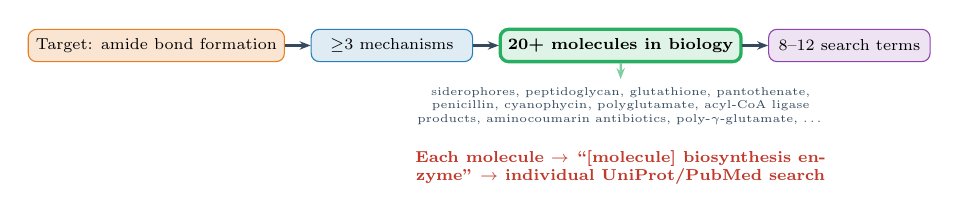
\begin{tikzpicture}[
    scale=0.82, transform shape,
    node distance=0.3cm,
    box/.style={rectangle, rounded corners=3pt, minimum height=0.5cm, text centered, font=\scriptsize, draw},
    arr/.style={-{Stealth[length=4pt]}, thick, color=darkgray},
]

% Flow: Target bond → Molecule enumeration → Search terms → Broad coverage
\node[box, fill=accentorange!20, draw=accentorange, minimum width=2.8cm] (target) {Target: amide bond formation};
\node[box, fill=accentblue!15, draw=accentblue, right=0.4cm of target, minimum width=2.5cm] (mech) {$\geq$3 mechanisms};
\node[box, fill=accentgreen!15, draw=accentgreen, right=0.4cm of mech, minimum width=3.0cm, line width=1.2pt] (mol) {\textbf{20+ molecules in biology}};
\node[box, fill=softpurple!15, draw=softpurple, right=0.4cm of mol, minimum width=2.5cm] (search) {8--12 search terms};

\draw[arr] (target) -- (mech);
\draw[arr] (mech) -- (mol);
\draw[arr] (mol) -- (search);

% Molecule examples fanning out below
\node[font=\tiny\color{darkgray}, below=0.25cm of mol, text width=6.5cm, align=center] (examples) {
siderophores, peptidoglycan, glutathione, pantothenate, penicillin, cyanophycin, polyglutamate, acyl-CoA ligase products, aminocoumarin antibiotics, poly-$\gamma$-glutamate, \ldots
};

\draw[arr, dashed, color=accentgreen!60] (mol.south) -- (examples.north);

% Key insight
\node[font=\scriptsize\color{accentred}\bfseries, below=0.15cm of examples, text width=8cm, align=center] {
Each molecule $\rightarrow$ ``[molecule] biosynthesis enzyme'' $\rightarrow$ individual UniProt/PubMed search
};

\end{tikzpicture}
\end{center}

\vspace{-2pt}
\begin{columns}[T]
\begin{column}{0.48\textwidth}
\begin{block}{\small Why This Drives Coverage}
\vspace{-2pt}
\begin{itemize}\scriptsize
\setlength\itemsep{1pt}
\item \textbf{Bond-type search is exhaustive}: every biological context where the target bond occurs is enumerated
\item Manual search typically covers 2--3 obvious pathways; the agent covers \textbf{all 6 biological contexts}: primary metabolism, cell wall, secondary metabolites, biopolymers, PTMs, xenobiotics
\item Each molecule name becomes a \textit{specific} search term, avoiding the ``long query returns 0 results'' trap
\end{itemize}
\end{block}
\end{column}
\begin{column}{0.48\textwidth}
\begin{exampleblock}{\small Steps A--D in Practice}
\vspace{-2pt}
\begin{itemize}\scriptsize
\setlength\itemsep{1pt}
\item \textbf{A.} Classify bond + direction; identify substrate analogues
\item \textbf{B.} Enumerate $\geq$3 distinct mechanisms with different folds (e.g., NIS synthetase, ANL adenylation, Gln synthetase fold)
\item \textbf{C.} List 20+ molecules containing the bond $\rightarrow$ recorded in notebook \texttt{enzyme\_landscape}
\item \textbf{D.} Write search specification \textit{before} any search tool call --- prevents ad hoc querying
\end{itemize}
\end{exampleblock}
\end{column}
\end{columns}
\end{frame}

% ════════════════════════════════════════════════════════════
% SLIDE 4c: Phase 2 Deep Dive — Multi-Axis Discovery
% ════════════════════════════════════════════════════════════
\begin{frame}{Phase 2: Discovery --- Four-Axis Database Search}
\vspace{-8pt}
\begin{center}
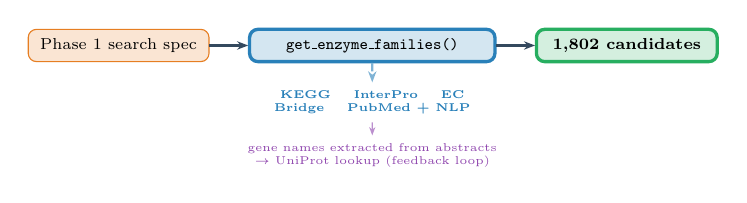
\begin{tikzpicture}[
    scale=0.82, transform shape,
    node distance=0.35cm,
    box/.style={rectangle, rounded corners=3pt, minimum height=0.5cm, text centered, font=\scriptsize, draw},
    arr/.style={-{Stealth[length=4pt]}, thick, color=darkgray},
]
\node[box, fill=accentorange!20, draw=accentorange, minimum width=2.8cm] (spec) {Phase 1 search spec};
\node[box, fill=accentblue!20, draw=accentblue, line width=1.2pt, minimum width=3.8cm, right=0.6cm of spec] (gef) {\texttt{get\_enzyme\_families()}};
\node[box, fill=accentgreen!20, draw=accentgreen, line width=1.2pt, minimum width=2.8cm, right=0.6cm of gef] (out) {\textbf{1,802 candidates}};
\draw[arr] (spec) -- (gef);
\draw[arr] (gef) -- (out);
\node[font=\tiny\bfseries\color{accentblue}, below=0.3cm of gef, text width=5.5cm, align=center] (axes)
    {KEGG \quad InterPro \quad EC Bridge \quad PubMed + NLP};
\draw[arr, dashed, color=accentblue!60] (gef.south) -- (axes.north);
\node[font=\tiny\color{softpurple}, below=0.2cm of axes, text width=5.5cm, align=center] (fb)
    {gene names extracted from abstracts $\rightarrow$ UniProt lookup (feedback loop)};
\draw[-{Stealth[length=3pt]}, color=softpurple!60, dashed] (axes.south) -- (fb.north);
\end{tikzpicture}
\end{center}

\vspace{-2pt}
\begin{columns}[T]
\begin{column}{0.48\textwidth}
\begin{block}{\small Four Search Axes}
\vspace{-2pt}
\begin{itemize}\scriptsize
\setlength\itemsep{1pt}
\item \textbf{KEGG}: enumerate all EC entries per prefix; auto-generate PubMed queries from KEGG enzyme names, bypassing LLM keyword quality
\item \textbf{InterPro}: keyword search returning family IDs + full member-list enrichment
\item \textbf{EC Bridge}: samples UniProt entries across all EC\,6.x ligases --- catches rare classes with no keyword match (e.g., EC\,6.3.2.29, EC\,6.3.2.59)
\item \textbf{PubMed + NLP}: entity extraction returns gene names invisible to keyword search; new names fed back to UniProt
\end{itemize}
\end{block}
\end{column}
\begin{column}{0.48\textwidth}
\begin{exampleblock}{\small Why Not Just EC Numbers?}
\vspace{-2pt}
\begin{itemize}\scriptsize
\setlength\itemsep{1pt}
\item Novel biosynthetic enzymes (e.g., DdaG, SfaB) often lack an assigned EC number at the time of discovery
\item Substrate-based and domain-based axes capture these unannotated entries
\item EC Bridge is exhaustive: scans every ligase subclass, not just sampled prefixes; the only axis that finds pyrrolysine ligase (EC\,6.3.2.59)
\item Gene names from paper abstracts provide the most specific UniProt key --- direct sequence match without ambiguity
\end{itemize}
\end{exampleblock}
\end{column}
\end{columns}
\end{frame}

% ════════════════════════════════════════════════════════════
% SLIDE 4d: Phase 3 Deep Dive — Candidate Evaluation
% ════════════════════════════════════════════════════════════
\begin{frame}{Phase 3: Candidate Evaluation --- Gates, Hard Limits, and Structured Scoring}
\vspace{-14pt}
\begin{center}
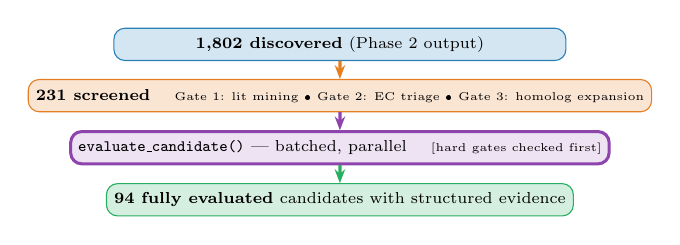
\begin{tikzpicture}[
    scale=0.82, transform shape,
    node distance=0.25cm,
    box/.style={rectangle, rounded corners=4pt, text centered, font=\scriptsize, draw, minimum height=0.5cm},
    arr/.style={-{Stealth[length=5pt]}, very thick},
]
\node[box, fill=accentblue!20, draw=accentblue, minimum width=7cm] (d)
    {\textbf{1,802 discovered} (Phase 2 output)};
\node[box, fill=accentorange!20, draw=accentorange, minimum width=7cm, below=0.28cm of d] (s)
    {\textbf{231 screened} \quad{\normalfont\tiny Gate 1: lit mining \textbullet\ Gate 2: EC triage \textbullet\ Gate 3: homolog expansion}};
\node[box, fill=softpurple!15, draw=softpurple, line width=1.1pt, minimum width=7cm, below=0.28cm of s] (e)
    {\texttt{evaluate\_candidate()} --- batched, parallel \quad{\normalfont\tiny[hard gates checked first]}};
\node[box, fill=accentgreen!20, draw=accentgreen, minimum width=7cm, below=0.28cm of e] (out)
    {\textbf{94 fully evaluated} candidates with structured evidence};
\draw[arr, color=accentorange] (d) -- (s);
\draw[arr, color=softpurple] (s) -- (e);
\draw[arr, color=accentgreen] (e) -- (out);
\end{tikzpicture}
\end{center}

\vspace{-8pt}
\begin{columns}[T]
\begin{column}{0.48\textwidth}
\begin{alertblock}{\small Hard vs.\ Soft Gates}
\vspace{-2pt}
\begin{itemize}\scriptsize
\setlength\itemsep{0pt}
\item \textbf{Hard} (require PMID to override): bond-type mismatch, direction mismatch (formation vs.\ cleavage), severe size mismatch ($>6.7\times$ MW) --- thermodynamic constraints
\item \textbf{Soft} (LLM weighs contextually): moderate size mismatch, low characterization, TrEMBL auto-annotation only
\item \texttt{evaluate\_candidate()} returns \textbf{raw facts only}; no composite score --- LLM applies biochemical judgment
\end{itemize}
\end{alertblock}
\end{column}
\begin{column}{0.48\textwidth}
\begin{exampleblock}{\small Per-Substrate Scoring Hierarchy}
\vspace{-2pt}
\begin{itemize}\scriptsize
\setlength\itemsep{0pt}
\item \textbf{1st:} Functional group counts (carboxyl, amine, hydroxyl, thiol) --- most direct substrate compatibility signal
\item \textbf{2nd:} MW similarity, chain length, LogP, TPSA
\item \textbf{3rd:} Tanimoto fingerprint (ECFP4) --- can be misleading in isolation
\item Multi-substrate: geometric mean; $>3\times$ ratio flags discordance
\end{itemize}
\end{exampleblock}
\end{column}
\end{columns}
\end{frame}

% ════════════════════════════════════════════════════════════
% SLIDE 4e: Phase 4 Deep Dive — Ranking & Report
% ════════════════════════════════════════════════════════════
\begin{frame}{Phase 4: Ranking \& Report --- Evidence to Recommendations}
\vspace{-12pt}
\begin{columns}[T]
\begin{column}{0.48\textwidth}
\begin{block}{\small 4-Level Ranking Framework}
\vspace{-2pt}
\begin{itemize}\scriptsize
\setlength\itemsep{1pt}
\item \textbf{P0.} {\color{accentred}Critical warning} $\rightarrow$ bottom tier, no promotion
\item \textbf{P1.} Substrate compatibility: FG counts $>$ MW $>$ Tanimoto
\item \textbf{P2.} Characterization: Swiss-Prot curation + $\geq$5 mechanism papers
\item \textbf{P3.} Structure: PDB crystal $>$ AlphaFold $>$ none
\item \textbf{P4.} Engineering: $\geq$2 directed evolution or design papers
\end{itemize}
\end{block}

\vspace{1pt}
\begin{alertblock}{\small Why No Composite Score?}
\vspace{-2pt}
\begin{itemize}\scriptsize
\setlength\itemsep{0pt}
\item Weights are brittle: a 0.4 Tanimoto with the correct bond-forming mechanism may outrank a 0.9 Tanimoto with the wrong reaction direction
\item P0--P4 define ordering logic; LLM provides biochemical judgment within each tier
\end{itemize}
\end{alertblock}
\end{column}
\begin{column}{0.48\textwidth}
\begin{exampleblock}{\small Dual Report Strategy}
\vspace{-2pt}
\begin{itemize}\scriptsize
\setlength\itemsep{0pt}
\item \textbf{Report 1 (confidence-weighted)}: rank by experimental evidence --- Swiss-Prot curation, crystal structures, kinetic data; conservative engineering use case
\item \textbf{Report 2 (suitability-focused)}: rank by biochemical fit --- substrate chemistry, mechanism, potential; evidence as separate \textit{Confidence} column that does \textbf{not} affect rank; exploratory use case
\item Same data, different ranking --- under-characterized enzymes with excellent substrate match surface only in Report 2
\end{itemize}
\end{exampleblock}

\vspace{1pt}
\begin{block}{\small Artifacts Generated}
\vspace{-2pt}
\begin{itemize}\scriptsize
\setlength\itemsep{0pt}
\item \texttt{report\_confidence.md} + \texttt{report\_explorative.md}
\item \texttt{candidates.csv} (94 evaluated, structured columns)
\item PDB / AlphaFold structure files (Tier\,1 candidates)
\item \texttt{events.jsonl} (structured audit trail)
\end{itemize}
\end{block}
\end{column}
\end{columns}
\end{frame}

% ════════════════════════════════════════════════════════════
% SLIDE 5: Agent Loop + Key Mechanisms
% ════════════════════════════════════════════════════════════
\begin{frame}{Agent Loop --- Core Mechanics}
\begin{center}
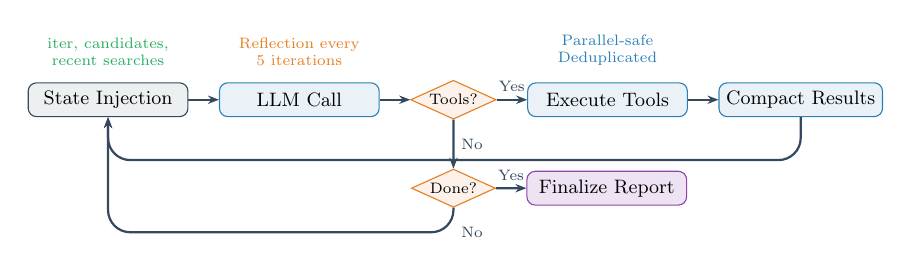
\begin{tikzpicture}[
    scale=0.78, transform shape,
    node distance=0.5cm,
    every node/.style={font=\small},
    procstep/.style={rectangle, rounded corners=3pt, minimum width=2.6cm, minimum height=0.55cm, text centered, draw=accentblue, fill=accentblue!10, font=\small},
    gate/.style={diamond, aspect=2.2, minimum width=1.3cm, draw=accentorange, fill=accentorange!10, font=\scriptsize, inner sep=1pt},
    arr/.style={-{Stealth[length=4pt]}, thick, color=darkgray},
]

% Main flow (horizontal)
\node[procstep, fill=lightgray, draw=darkgray] (state) {State Injection};
\node[procstep, right=0.5cm of state] (llm) {LLM Call};
\node[gate, right=0.5cm of llm] (tools) {Tools?};
\node[procstep, right=0.5cm of tools] (exec) {Execute Tools};
\node[procstep, right=0.5cm of exec] (result) {Compact Results};

% Return arrow
\draw[arr] (state) -- (llm);
\draw[arr] (llm) -- (tools);
\draw[arr] (tools) -- node[above, font=\scriptsize] {Yes} (exec);
\draw[arr] (exec) -- (result);
\draw[arr, rounded corners=8pt] (result.south) -- ++(0,-0.7) -| (state.south);

% No tools path
\node[gate, below=0.8cm of tools] (done) {Done?};
\draw[arr] (tools) -- node[right, font=\scriptsize] {No} (done);

\node[procstep, fill=softpurple!15, draw=softpurple, right=0.5cm of done] (report) {Finalize Report};
\draw[arr] (done) -- node[above, font=\scriptsize] {Yes} (report);

% Continue
\draw[arr, rounded corners=8pt] (done.south) -- ++(0,-0.4) node[right, font=\scriptsize] {No} -| (state.south);

% Annotations
\node[font=\scriptsize\color{accentgreen}, above=0.15cm of state, align=center] {iter, candidates,\\recent searches};
\node[font=\scriptsize\color{accentorange}, above=0.15cm of llm, align=center] {Reflection every\\5 iterations};
\node[font=\scriptsize\color{accentblue}, above=0.15cm of exec, align=center, text width=2.3cm] {\scriptsize Parallel-safe\\Deduplicated};

\end{tikzpicture}
\end{center}

\vspace{4pt}
\begin{columns}[T]
\begin{column}{0.48\textwidth}
\begin{block}{\small Key Features}
\begin{itemize}\scriptsize
\item \textbf{State injection} every iteration (progress, phase)
\item \textbf{Reflection} every 5 iterations (coverage gaps)
\item \textbf{Search deduplication} prevents redundant queries
\item \textbf{Anti-early-termination} gates
\end{itemize}
\end{block}
\end{column}
\begin{column}{0.48\textwidth}
\begin{block}{\small Artifact Management}
\begin{itemize}\scriptsize
\item Results saved as JSON artifacts by category
\item Bulky fields stripped for LLM context (\texttt{\_compact\_for\_llm})
\item Full data preserved in \texttt{artifacts/} directory
\item Structured event log (\texttt{events.jsonl})
\end{itemize}
\end{block}
\end{column}
\end{columns}
\end{frame}

% ════════════════════════════════════════════════════════════
% SLIDE 6: Tool Ecosystem + Usage Data (merged)
% ════════════════════════════════════════════════════════════
\begin{frame}{Tool Ecosystem --- 18 Tools Across 6 Categories}
\vspace{-4pt}

\begin{columns}[T]
\begin{column}{0.32\textwidth}

\begin{block}{\faMortarPestle\ \ Chemistry (3)}
\begin{itemize}\scriptsize
\setlength\itemsep{0pt}
\item \texttt{validate\_smiles}
\item \texttt{get\_mol\_properties}
\item \texttt{fingerprint\_similarity}
\end{itemize}
\end{block}

\begin{block}{\faDatabase\ \ Database (5)}
\begin{itemize}\scriptsize
\setlength\itemsep{0pt}
\item \texttt{search\_uniprot}
\item \texttt{fetch\_uniprot\_seq}
\item \texttt{search\_kegg\_enzyme}
\item \texttt{search\_interpro}
\item \texttt{get\_protein\_domains}
\end{itemize}
\end{block}

\end{column}
\begin{column}{0.32\textwidth}

\begin{block}{\faBook\ \ Literature (4)}
\begin{itemize}\scriptsize
\setlength\itemsep{0pt}
\item \texttt{search\_pubmed}
\item \texttt{search\_openalex}
\item \texttt{extract\_entities}
\item \texttt{deep\_lit\_search}
\end{itemize}
\end{block}

\begin{block}{\faFlask\ \ Substrate (1)}
\begin{itemize}\scriptsize
\setlength\itemsep{0pt}
\item \texttt{analyze\_substrate}
\end{itemize}
\end{block}

\end{column}
\begin{column}{0.32\textwidth}

\begin{block}{\faBrain\ \ Reasoning (4)}
\begin{itemize}\scriptsize
\setlength\itemsep{0pt}
\item \texttt{update\_notebook}
\item \texttt{get\_notebook}
\item \texttt{evaluate\_candidate}
\item \texttt{screen\_candidates}
\end{itemize}
\end{block}

\begin{block}{\faCubes\ \ Structure I/O (1)}
\begin{itemize}\scriptsize
\setlength\itemsep{0pt}
\item \texttt{load\_structure\_file}
\end{itemize}
\end{block}

\end{column}
\end{columns}

\vspace{2pt}
\begin{center}
\colorbox{lightblue!50}{\parbox{0.92\textwidth}{\centering
\scriptsize \texttt{@tool} decorator auto-generates OpenAI function-calling schema from Python type hints.
Parallel-safe tools execute concurrently (4-thread pool). Results compacted for LLM context (abstracts $\rightarrow$ 200\,chars, lists $\rightarrow$ 8--10 items); full data preserved in \texttt{artifacts/} directory.
}}
\end{center}
\end{frame}

% ════════════════════════════════════════════════════════════
% SLIDE 7: Pre-Evaluation Gates (3 gates)
% ════════════════════════════════════════════════════════════
\begin{frame}{Automated Pre-Evaluation Gates}
\vspace{-4pt}
\begin{center}
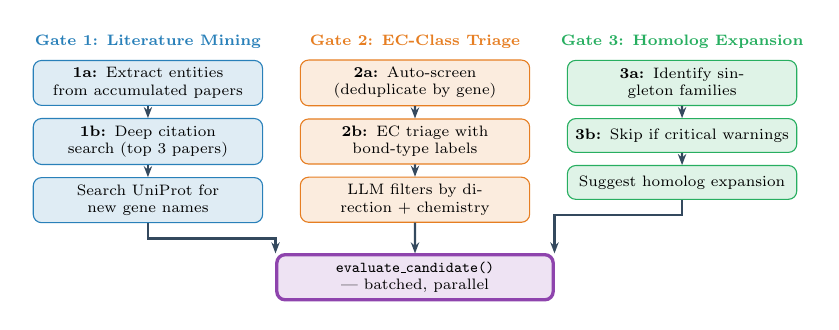
\begin{tikzpicture}[
    scale=0.78, transform shape,
    node distance=0.25cm,
    box/.style={rectangle, rounded corners=3pt, minimum height=0.55cm, text centered, font=\scriptsize, text width=3.5cm, draw},
    arr/.style={-{Stealth[length=4pt]}, thick, color=darkgray},
]

% Gate 1
\node[box, fill=accentblue!15, draw=accentblue] (g1a) {\textbf{1a:} Extract entities from accumulated papers};
\node[box, fill=accentblue!15, draw=accentblue, below=0.2cm of g1a] (g1b) {\textbf{1b:} Deep citation search (top 3 papers)};
\node[box, fill=accentblue!15, draw=accentblue, below=0.2cm of g1b] (g1c) {Search UniProt for new gene names};

% Gate 2
\node[box, fill=accentorange!15, draw=accentorange, right=0.6cm of g1a] (g2a) {\textbf{2a:} Auto-screen (deduplicate by gene)};
\node[box, fill=accentorange!15, draw=accentorange, below=0.2cm of g2a] (g2b) {\textbf{2b:} EC triage with bond-type labels};
\node[box, fill=accentorange!15, draw=accentorange, below=0.2cm of g2b] (g2c) {LLM filters by direction + chemistry};

% Gate 3
\node[box, fill=accentgreen!15, draw=accentgreen, right=0.6cm of g2a] (g3a) {\textbf{3a:} Identify singleton families};
\node[box, fill=accentgreen!15, draw=accentgreen, below=0.2cm of g3a] (g3b) {\textbf{3b:} Skip if critical warnings};
\node[box, fill=accentgreen!15, draw=accentgreen, below=0.2cm of g3b] (g3c) {Suggest homolog expansion};

% Evaluate
\node[box, fill=softpurple!15, draw=softpurple, line width=1.2pt, below=0.5cm of g2c, minimum width=4.5cm] (eval) {\texttt{evaluate\_candidate()} --- batched, parallel};

% Arrows
\draw[arr] (g1a) -- (g1b);
\draw[arr] (g1b) -- (g1c);
\draw[arr] (g2a) -- (g2b);
\draw[arr] (g2b) -- (g2c);
\draw[arr] (g3a) -- (g3b);
\draw[arr] (g3b) -- (g3c);
\draw[arr] (g1c.south) -- ++(0,-0.25) -| (eval.north west);
\draw[arr] (g2c) -- (eval);
\draw[arr] (g3c.south) -- ++(0,-0.25) -| (eval.north east);

% Labels
\node[font=\scriptsize\bfseries\color{accentblue}, above=0.06cm of g1a] {Gate 1: Literature Mining};
\node[font=\scriptsize\bfseries\color{accentorange}, above=0.06cm of g2a] {Gate 2: EC-Class Triage};
\node[font=\scriptsize\bfseries\color{accentgreen}, above=0.06cm of g3a] {Gate 3: Homolog Expansion};

\end{tikzpicture}
\end{center}

\vspace{-4pt}
{\centering\scriptsize\color{darkgray} Gates trigger automatically when the LLM first calls \texttt{evaluate\_candidate}\par}
\vspace{2pt}

\begin{columns}[T]
\begin{column}{0.32\textwidth}
\begin{block}{\scriptsize Gate 1}
\vspace{-2pt}
\begin{itemize}\scriptsize
\setlength\itemsep{0pt}
\item NLP entity extraction: gene names, EC numbers, families
\item Follow citation networks (refs of refs)
\item Inject new search terms before evaluation
\end{itemize}
\end{block}
\end{column}
\begin{column}{0.32\textwidth}
\begin{block}{\scriptsize Gate 2}
\vspace{-2pt}
\begin{itemize}\scriptsize
\setlength\itemsep{0pt}
\item Pre-compute bond-type per candidate via 52-entry IUBMB EC map
\item Present as: ``\textbf{FORMS} amide'' / ``\textbf{CLEAVES} amide''
\item LLM excludes direction mismatches
\end{itemize}
\end{block}
\end{column}
\begin{column}{0.32\textwidth}
\begin{block}{\scriptsize Gate 3}
\vspace{-2pt}
\begin{itemize}\scriptsize
\setlength\itemsep{0pt}
\item Families with 1 evaluated member and \textbf{no} critical warnings
\item Suggest InterPro homolog search
\item Skip families with bond-type mismatch
\end{itemize}
\end{block}
\end{column}
\end{columns}
\end{frame}

% ════════════════════════════════════════════════════════════
% SLIDE 7b: Candidate Evaluation Framework
% ════════════════════════════════════════════════════════════
\begin{frame}{Candidate Evaluation Framework}
\vspace{-6pt}

\begin{columns}[T]
\begin{column}{0.48\textwidth}

% Bond-type validation
\begin{alertblock}{\small Critical Warnings (Hard Gates)}
\vspace{-2pt}
\begin{itemize}\scriptsize
\setlength\itemsep{1pt}
\item \textbf{Bond-type mismatch}: 52-entry IUBMB EC $\rightarrow$ bond-type map classifies every enzyme's native chemistry
\item \textbf{Reaction direction mismatch}: formation vs.\ cleavage (thermodynamically irreversible without cofactor change)
\item \textbf{Severe size mismatch}: MW ratio $>$\,6.7$\times$ (similarity $<$\,0.15)
\end{itemize}
\vspace{1pt}
{\tiny\color{accentred} Cannot be overridden without specific PMID demonstrating target reaction}
\end{alertblock}

\vspace{2pt}
% Substrate class detection
\begin{block}{\small Substrate Classification}
\vspace{-2pt}
\begin{itemize}\scriptsize
\setlength\itemsep{1pt}
\item \textbf{Polymer}: detects \texttt{(n)}, \texttt{poly-}, NRPS/PKS domains
\item \textbf{Carrier-tethered}: ACP, ArCP, pantetheine
\item \textbf{Peptide vs.\ amide}: EC 3.4 $\neq$ EC 3.5
\item \textbf{Cofactors}: extracts \texttt{required\_cofactors} from UniProt
\end{itemize}
\end{block}

\end{column}
\begin{column}{0.48\textwidth}

% Per-substrate scoring
\begin{exampleblock}{\small Per-Substrate Scoring}
\vspace{-2pt}
\begin{itemize}\scriptsize
\setlength\itemsep{1pt}
\item Each target substrate scored independently
\item \textbf{Primary}: functional group counts (carboxyl, amine, hydroxyl, thiol)
\item \textbf{Secondary}: MW similarity, chain length, LogP, TPSA
\item \textbf{Reference}: Tanimoto fingerprint (ECFP4)
\item Multi-substrate: geometric mean with one-sided mismatch detection (ratio $>$\,3$\times$)
\end{itemize}
\end{exampleblock}

\vspace{2pt}
% Ranking framework
\begin{block}{\small 4-Level Ranking Framework}
\vspace{-2pt}
\begin{itemize}\scriptsize
\setlength\itemsep{0pt}
\item \textbf{P0.} {\color{accentred}\textbf{Critical warnings}} $\rightarrow$ bottom tier (hard gate)
\item \textbf{P1.} \textbf{Substrate compatibility} (FG counts $>$ MW $>$ Tanimoto)
\item \textbf{P2.} \textbf{Characterization depth} (Swiss-Prot curation, $\geq$5 kinetics/mechanism papers)
\item \textbf{P3.} \textbf{Structural data} (PDB $>$ AlphaFold $>$ none)
\item \textbf{P4.} \textbf{Engineering precedent} ($\geq$2 directed evolution / rational design papers)
\end{itemize}
\end{block}

\end{column}
\end{columns}
\end{frame}

% ════════════════════════════════════════════════════════════
% SLIDE 8b: Literature Mining Pipeline
% ════════════════════════════════════════════════════════════
\begin{frame}{Literature Mining Pipeline}
\vspace{-6pt}
\begin{center}
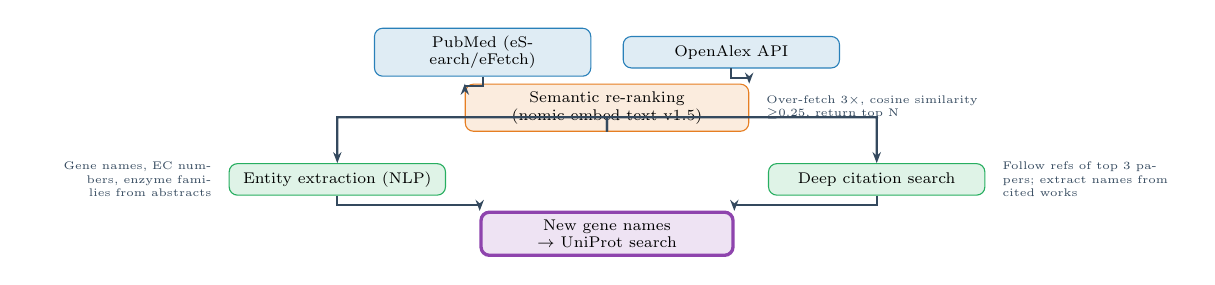
\begin{tikzpicture}[
    scale=0.80, transform shape,
    node distance=0.3cm,
    box/.style={rectangle, rounded corners=3pt, minimum height=0.5cm, text centered, font=\scriptsize, draw, text width=3.2cm},
    arr/.style={-{Stealth[length=4pt]}, thick, color=darkgray},
]

% Row 1: Search sources
\node[box, fill=accentblue!15, draw=accentblue] (pm) {PubMed (eSearch/eFetch)};
\node[box, fill=accentblue!15, draw=accentblue, right=0.5cm of pm] (oa) {OpenAlex API};

% Row 2: Over-fetch + Re-rank
\node[box, fill=accentorange!15, draw=accentorange, below=0.5cm of $(pm)!0.5!(oa)$, minimum width=4.5cm] (rerank) {Semantic re-ranking (nomic-embed-text-v1.5)};

% Row 3: Entity extraction + Deep search
\node[box, fill=accentgreen!15, draw=accentgreen, below left=0.5cm and 0.3cm of rerank] (entity) {Entity extraction (NLP)};
\node[box, fill=accentgreen!15, draw=accentgreen, below right=0.5cm and 0.3cm of rerank] (deep) {Deep citation search};

% Row 4: New genes
\node[box, fill=softpurple!15, draw=softpurple, below=0.5cm of $(entity)!0.5!(deep)$, minimum width=4.0cm, line width=1.2pt] (genes) {New gene names $\rightarrow$ UniProt search};

% Arrows
\draw[arr] (pm.south) -- ++(0,-0.15) -| (rerank.north west);
\draw[arr] (oa.south) -- ++(0,-0.15) -| (rerank.north east);
\draw[arr] (rerank) -- ++(0,-0.15) -| (entity.north);
\draw[arr] (rerank) -- ++(0,-0.15) -| (deep.north);
\draw[arr] (entity.south) -- ++(0,-0.15) -| (genes.north west);
\draw[arr] (deep.south) -- ++(0,-0.15) -| (genes.north east);

% Annotations
\node[font=\tiny\color{darkgray}, right=0.15cm of rerank, text width=3.5cm, align=left] {Over-fetch 3$\times$, cosine similarity $\geq$0.25, return top N};
\node[font=\tiny\color{darkgray}, left=0.15cm of entity, text width=2.8cm, align=right] {Gene names, EC numbers, enzyme families from abstracts};
\node[font=\tiny\color{darkgray}, right=0.15cm of deep, text width=2.8cm, align=left] {Follow refs of top 3 papers; extract names from cited works};

\end{tikzpicture}
\end{center}

\vspace{-2pt}
\begin{columns}[T]
\begin{column}{0.48\textwidth}
\begin{alertblock}{\small Why Citation Mining Matters}
\vspace{-2pt}
\begin{itemize}\scriptsize
\setlength\itemsep{1pt}
\item Abstracts often \textbf{lack specific gene names} --- those appear only in full text
\item Referenced papers have those names in their \textit{own} titles/abstracts
\item This is how the agent discovers enzymes \textbf{invisible to keyword search}
\end{itemize}
\end{alertblock}
\end{column}
\begin{column}{0.48\textwidth}
\begin{block}{\small Search Deduplication}
\vspace{-2pt}
\begin{itemize}\scriptsize
\setlength\itemsep{1pt}
\item Similarity = max(Jaccard\textsubscript{tokens}, SequenceMatcher\textsubscript{chars})
\item Threshold $\geq$0.90 $\rightarrow$ return cached result
\item Prevents wasting iterations on near-identical queries
\item Applies to all literature + database search tools
\end{itemize}
\end{block}
\end{column}
\end{columns}
\end{frame}

% ════════════════════════════════════════════════════════════
% SLIDE 8c: Dual Report System
% ════════════════════════════════════════════════════════════
\begin{frame}{Output: Dual-Ranked Reports}
\vspace{-4pt}
\begin{columns}[T]
\begin{column}{0.48\textwidth}

\begin{block}{\small Confidence-Weighted Report}
\vspace{-2pt}
\begin{itemize}\scriptsize
\setlength\itemsep{1pt}
\item \textbf{Ranking criterion}: experimental evidence drives position
\item Swiss-Prot curation, characterization papers, crystal structures $\rightarrow$ higher rank
\item \textbf{Use case}: conservative engineering --- start with the most well-understood enzyme
\item Generated in-run (LLM produces report when it stops calling tools)
\end{itemize}
\end{block}

\begin{exampleblock}{\small Shared Report Structure}
\vspace{-2pt}
\begin{itemize}\scriptsize
\setlength\itemsep{0pt}
\item Executive Summary (target, families, top candidate + why)
\item Enzyme Families Discovered (table)
\item Candidate Table (all candidates, one table)
\item Tier 1 Profiles (detailed per candidate)
\item Key Literature References
\end{itemize}
\end{exampleblock}

\end{column}
\begin{column}{0.48\textwidth}

\begin{alertblock}{\small Suitability-Focused (Explorative) Report}
\vspace{-2pt}
\begin{itemize}\scriptsize
\setlength\itemsep{1pt}
\item \textbf{Ranking criterion}: biochemical suitability drives position
\item Substrate chemistry match, mechanism compatibility, engineering potential $\rightarrow$ higher rank
\item Evidence $\rightarrow$ separate \textbf{Confidence column} (High/Med/Low) that does \textbf{NOT} affect rank
\item \textbf{Use case}: exploratory discovery --- find the biochemically closest enzyme, even if under-studied
\end{itemize}
\end{alertblock}

\vspace{2pt}
\begin{center}
\colorbox{lightblue!50}{\parbox{0.92\textwidth}{\centering
\scriptsize\textbf{Why two reports?} The same evaluation data, ranked by different criteria, surfaces \textbf{different candidates}. Under-characterized enzymes with excellent substrate match appear in the explorative report but not the confidence report --- highlighting priorities for experimental validation.
}}
\end{center}

\end{column}
\end{columns}
\end{frame}

% ════════════════════════════════════════════════════════════
% SLIDE 9: Test Run Overview (section divider)
% ════════════════════════════════════════════════════════════
{
\setbeamercolor{background canvas}{bg=accentblue!90!black}
\begin{frame}[plain]
\vfill
\begin{center}
{\Large\bfseries\color{white} Test Runs: Polyamide Enzyme Discovery}\\[10pt]
{\large\color{lightblue!80} Four queries spanning aliphatic and aromatic substrates}\\[16pt]
\colorbox{white!95}{\begin{minipage}{0.92\textwidth}
\centering\small
\begin{tabular}{@{}c p{5.5cm} l l c@{}}
\toprule
\textbf{\#} & \textbf{Query} & \textbf{Reaction} & \textbf{Substrates} & \textbf{Status}\\
\midrule
1 & Aliphatic amide formation & ATP-dep.\ ligation & Adipic acid + HMD & Completed\\
2 & Nylon-66 hydrolysis & Amide hydrolysis & Nylon-66 oligomers & Completed\\
3 & PPTA synthesis (para) & ATP-dep.\ ligation & TPA + PPD & Completed\\
4 & PMIA synthesis (meta) & ATP-dep.\ ligation & IPA + MPD & Completed\\
\bottomrule
\end{tabular}
\end{minipage}}
\\[12pt]
{\small\color{white!80} All runs fully autonomous --- Claude Sonnet 4.6 via Argo API}
\end{center}
\vfill
\end{frame}
}

% ════════════════════════════════════════════════════════════
% SLIDE 9: Per-Run Statistics + Funnel (merged)
% ════════════════════════════════════════════════════════════
\begin{frame}{Discovery at Scale}
\vspace{-6pt}

\begin{columns}[T]
\begin{column}{0.48\textwidth}

% Discovery funnel visualization
\begin{center}
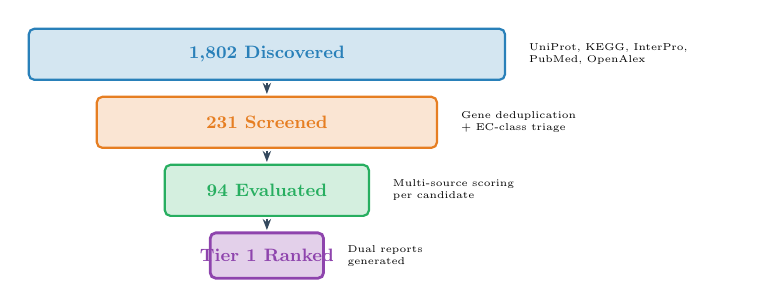
\begin{tikzpicture}[scale=0.72, transform shape]
% Funnel bars (narrowing)
\fill[accentblue!20, draw=accentblue, line width=0.8pt, rounded corners=2pt]
    (-4.2,0) -- (4.2,0) -- (4.2,0.9) -- (-4.2,0.9) -- cycle;
\fill[accentorange!20, draw=accentorange, line width=0.8pt, rounded corners=2pt]
    (-3.0,-1.2) -- (3.0,-1.2) -- (3.0,-0.3) -- (-3.0,-0.3) -- cycle;
\fill[accentgreen!20, draw=accentgreen, line width=0.8pt, rounded corners=2pt]
    (-1.8,-2.4) -- (1.8,-2.4) -- (1.8,-1.5) -- (-1.8,-1.5) -- cycle;
\fill[softpurple!25, draw=softpurple, line width=1pt, rounded corners=2pt]
    (-1.0,-3.5) -- (1.0,-3.5) -- (1.0,-2.7) -- (-1.0,-2.7) -- cycle;

\node[font=\small\bfseries] at (0, 0.45) {\color{accentblue}1{,}802 Discovered};
\node[font=\small\bfseries] at (0, -0.75) {\color{accentorange}231 Screened};
\node[font=\small\bfseries] at (0, -1.95) {\color{accentgreen}94 Evaluated};
\node[font=\small\bfseries] at (0, -3.1) {\color{softpurple}Tier 1 Ranked};

% Right annotations
\node[font=\tiny, anchor=west, text width=3.5cm] at (4.5, 0.45) {UniProt, KEGG, InterPro,\\PubMed, OpenAlex};
\node[font=\tiny, anchor=west, text width=3.5cm] at (3.3, -0.75) {Gene deduplication\\+ EC-class triage};
\node[font=\tiny, anchor=west, text width=3.5cm] at (2.1, -1.95) {Multi-source scoring\\per candidate};
\node[font=\tiny, anchor=west, text width=3.5cm] at (1.3, -3.1) {Dual reports\\generated};

% Arrows
\draw[-{Stealth[length=4pt]}, thick, color=darkgray] (0,-0.05) -- (0,-0.25);
\draw[-{Stealth[length=4pt]}, thick, color=darkgray] (0,-1.25) -- (0,-1.45);
\draw[-{Stealth[length=4pt]}, thick, color=darkgray] (0,-2.45) -- (0,-2.65);
\end{tikzpicture}
\end{center}

\end{column}
\begin{column}{0.48\textwidth}

\begin{center}
\includegraphics[width=\textwidth]{figs/discovery_bars.pdf}
\end{center}

\vspace{-4pt}
\begin{center}
\scriptsize 89 iterations $\cdot$ 94 evaluated $\cdot$ 9.1\,M tokens
\end{center}

\end{column}
\end{columns}
\end{frame}

% ════════════════════════════════════════════════════════════
% SLIDE 10: Run 1 — Aliphatic Amide Formation
% ════════════════════════════════════════════════════════════
\begin{frame}{Run 1: Aliphatic Amide Formation}
\vspace{-8pt}
\begin{center}
\scriptsize\color{darkgray} \textit{Adipic acid + hexamethylenediamine $\rightarrow$ amide (ATP-dependent)}
\end{center}
\vspace{-4pt}

{\scriptsize
\begin{adjustbox}{max width=\textwidth}
\begin{tabular}{@{}c l l l l p{5.5cm}@{}}
\toprule
\textbf{Rank} & \textbf{Gene} & \textbf{Family} & \textbf{Organism} & \textbf{Evidence} & \textbf{Key Rationale}\\
\midrule
1 & \texttt{asbA} & NIS synthetase & \textit{B.\,anthracis} & Swiss-Prot &
Perfect FG match on spermidine amine; documented diamine + diacid promiscuity\\
2 & \texttt{asbB} & NIS synthetase & \textit{B.\,anthracis} & PDB 3TO3, 4 mut. &
K313A/M variants accept linear diamines (HMD-like); best engineering tractability\\
3 & \texttt{puuA} & Gln syn.\ fold & \textit{E.\,coli} K12 & 2 mut., 2 eng. &
Highest Tanimoto (0.175); Glu MW = adipate; accepts cadaverine/spermidine\\
4 & \texttt{iucA} & NIS synthetase & \textit{E.\,coli} & 9 char.\ papers &
Well-characterized NIS; citrate acid substrate closest to adipic acid\\
5 & \texttt{iucC} & NIS synthetase & \textit{E.\,coli} & 19 char., 2 eng. &
Most-characterized NIS synthetase; standard reference enzyme\\
\bottomrule
\end{tabular}
\end{adjustbox}
}

\vspace{2pt}
\begin{columns}[T]
\begin{column}{0.48\textwidth}
\begin{exampleblock}{\scriptsize Dominant Families}
\vspace{-2pt}
\begin{itemize}\scriptsize
\setlength\itemsep{0pt}
\item \textbf{NIS synthetases} (IucA/IucC fold): 9 of 27 evaluated
\item \textbf{Gln synthetase fold} (PuuA): exact acid MW match
\item Also: ATP-grasp, cyanophycin syn., dapdiamide syn., MurC/D
\end{itemize}
\end{exampleblock}
\end{column}
\begin{column}{0.48\textwidth}
\begin{block}{\scriptsize Key Finding}
\vspace{-2pt}
\begin{itemize}\scriptsize
\setlength\itemsep{0pt}
\item NIS synthetases natively couple aliphatic diacids to diamines
\item AsbB mutagenesis demonstrates expandable amine scope
\item PuuA offers exact acid MW match (Glu 147\,Da $\approx$ adipate 146\,Da)
\item 18 distinct InterPro families across 27 candidates
\end{itemize}
\end{block}
\end{column}
\end{columns}
\end{frame}

% ════════════════════════════════════════════════════════════
% SLIDE 10b: Run 1 — Native Reaction Comparison
% ════════════════════════════════════════════════════════════
\begin{frame}{Run 1: Why AsbA/AsbB and PuuA Rank Highest}
\vspace{-6pt}

{\scriptsize
\begin{adjustbox}{max width=\textwidth}
\begin{tabular}{@{}r p{7.0cm} p{4.5cm}@{}}
\toprule
 & \textbf{Reaction} & \textbf{Key Substrates} \\
\midrule
\rowcolor{accentred!8}
\textbf{Target} & HOOC--(CH\textsubscript{2})\textsubscript{4}--COOH + H\textsubscript{2}N--(CH\textsubscript{2})\textsubscript{6}--NH\textsubscript{2} $\xrightarrow{\text{ATP}}$ amide & Adipic acid (C6 diacid, MW 146) + HMD (C6 diamine) \\[4pt]
\rowcolor{accentblue!8}
\textbf{\#1 AsbA} & Citrate + spermidine $\xrightarrow{\text{ATP}}$ petrobactin precursor & Diacid + triamine; documented diamine/diacid promiscuity \\[4pt]
\rowcolor{accentblue!8}
\textbf{\#2 AsbB} & Citryl-spermidine + spermidine $\xrightarrow{\text{ATP}}$ petrobactin & K313A/M mutants accept 1,8-diaminooctane (C8) \\[4pt]
\rowcolor{accentgreen!8}
\textbf{\#3 PuuA} & Glutamate + putrescine $\xrightarrow{\text{ATP}}$ $\gamma$-glutamylputrescine & Glu (MW 147 $\approx$ adipate) + C4 diamine \\
\bottomrule
\end{tabular}
\end{adjustbox}
}

\vspace{6pt}
\begin{columns}[T]
\begin{column}{0.48\textwidth}
\begin{block}{\scriptsize AsbA/AsbB: NIS Synthetases}
\vspace{-2pt}
\begin{itemize}\scriptsize
\setlength\itemsep{1pt}
\item Natively couple \textbf{diacid to diamine} via ATP --- same bond chemistry as target
\item AsbB K313A/M mutants accept 1,8-diaminooctane (C8), \textbf{bracketing HMD} (C6)
\item AsbA documented to accept diamine + dicarboxylate analogs
\end{itemize}
\end{block}
\end{column}
\begin{column}{0.48\textwidth}
\begin{block}{\scriptsize PuuA: Glutamine Synthetase Fold}
\vspace{-2pt}
\begin{itemize}\scriptsize
\setlength\itemsep{1pt}
\item Highest Tanimoto similarity (0.175) among all candidates
\item \textbf{Exact acid MW match}: glutamate (147\,Da) $\approx$ adipate (146\,Da)
\item Naturally accepts putrescine, cadaverine, spermidine (C4--C10)
\end{itemize}
\end{block}
\end{column}
\end{columns}
\end{frame}

% ════════════════════════════════════════════════════════════
% SLIDE 11: Run 2 — Nylon-66 Hydrolysis
% ════════════════════════════════════════════════════════════
\begin{frame}{Run 2: Nylon-66 Amide Bond Hydrolysis}
\vspace{-8pt}
\begin{center}
\scriptsize\color{darkgray} \textit{Hydrolysis of amide bonds in nylon-66 polymer or oligomers}
\end{center}
\vspace{-4pt}

{\scriptsize
\begin{adjustbox}{max width=\textwidth}
\begin{tabular}{@{}c l l l l p{5.5cm}@{}}
\toprule
\textbf{Rank} & \textbf{Gene} & \textbf{Family} & \textbf{Organism} & \textbf{Evidence} & \textbf{Key Rationale}\\
\midrule
1 & \texttt{nylC} & Ntn hydrolase & \textit{P.\,ureafaciens} & 11 PDB, 9 eng. &
Only enzyme with confirmed direct nylon-66 activity (EC 3.5.1.117)\\
2 & \texttt{nylB'} & $\beta$-lactamase & \textit{P.\,ureafaciens} & 19 PDB, 8 char. &
MW similarity 0.953 to nylon-66 dimer; gain-of-function mutations documented\\
3 & \texttt{nylB} & $\beta$-lactamase & \textit{P.\,ureafaciens} & 16 PDB &
Canonical nylon-6 dimer hydrolase (EC 3.5.1.46)\\
4 & \texttt{FAAH} & Amidase sig. & \textit{R.\,norvegicus} & 21 PDB &
Highest Tanimoto (0.667); long-chain aliphatic amides (C14--C24)\\
5 & \texttt{aam} & Amidase sig. & \textit{R.\,erythropolis} & 35 char. &
Only amidase with documented secondary (N-substituted) amide activity\\
\bottomrule
\end{tabular}
\end{adjustbox}
}

\vspace{2pt}
\begin{columns}[T]
\begin{column}{0.48\textwidth}
\begin{exampleblock}{\scriptsize Complete Degradation Pathway}
\vspace{-2pt}
\begin{itemize}\scriptsize
\setlength\itemsep{0pt}
\item \textbf{NylA} (EC 3.5.2.12): cyclic dimer hydrolase
\item \textbf{NylB} (EC 3.5.1.46): linear dimer hydrolase
\item \textbf{NylC} (EC 3.5.1.117): endo-oligomer hydrolase
\item All from \textit{P.\,ureafaciens} --- a complete pathway
\end{itemize}
\end{exampleblock}
\end{column}
\begin{column}{0.48\textwidth}
\begin{block}{\scriptsize Broader Families Explored}
\vspace{-2pt}
\begin{itemize}\scriptsize
\setlength\itemsep{0pt}
\item Amidase signature (FAAH, AmiE, Aam, urethanase)
\item Aliphatic amidases (4 candidates)
\item Cutinases, ceramidases, penicillin acylases
\item 11 families, 28 evaluated, 2.3\,M tokens
\end{itemize}
\end{block}
\end{column}
\end{columns}
\end{frame}

% ════════════════════════════════════════════════════════════
% SLIDE 11b: Run 2 — Native Reaction Comparison
% ════════════════════════════════════════════════════════════
\begin{frame}{Run 2: Why NylC Ranks Highest}
\vspace{-6pt}

{\scriptsize
\begin{adjustbox}{max width=\textwidth}
\begin{tabular}{@{}r p{7.5cm} p{4.0cm}@{}}
\toprule
 & \textbf{Substrate Structure} & \textbf{Bond Environment} \\
\midrule
\rowcolor{accentred!8}
\textbf{Target} & \ldots--CO--NH--(CH\textsubscript{2})\textsubscript{6}--NH--CO--(CH\textsubscript{2})\textsubscript{4}--CO--NH--\ldots\ + H\textsubscript{2}O & Nylon-66: alternating C6 diacid / C6 diamine \\[4pt]
\rowcolor{accentblue!8}
\textbf{\#1 NylC} & \ldots--CO--(CH\textsubscript{2})\textsubscript{5}--NH--CO--(CH\textsubscript{2})\textsubscript{5}--NH--\ldots\ + H\textsubscript{2}O & Nylon-6 oligomers: C5 self-condensation \\[4pt]
\rowcolor{accentorange!8}
\textbf{\#2 NylB'} & H\textsubscript{2}N--(CH\textsubscript{2})\textsubscript{5}--CO--NH--(CH\textsubscript{2})\textsubscript{5}--COOH + H\textsubscript{2}O & AHA dimer (MW sim.\ 0.953 to nylon-66 dimer) \\[4pt]
\rowcolor{accentgreen!8}
\textbf{\#4 FAAH} & Long-chain fatty acid amide + H\textsubscript{2}O & C14--C24 aliphatic amides (Tanimoto 0.667) \\
\bottomrule
\end{tabular}
\end{adjustbox}
}

\vspace{4pt}
{\centering\scriptsize\color{darkgray} NylC/NylB natively act on nylon-6 (C5), closely matching nylon-66 (C6 diacid / C6 diamine); FAAH acts on long-chain aliphatic amides\par}
\vspace{4pt}

\begin{columns}[T]
\begin{column}{0.48\textwidth}
\begin{exampleblock}{\scriptsize NylC + NylB': Best Matches}
\vspace{-2pt}
\begin{itemize}\scriptsize
\setlength\itemsep{0pt}
\item NylC: \textbf{endo-type}, confirmed nylon-66 activity; 11 PDB, 9 engineering papers
\item NylB': MW similarity 0.953; gain-of-function mutations (G181D, H266N) documented
\item NylB: canonical nylon-6 dimer hydrolase; 16 PDB structures
\end{itemize}
\end{exampleblock}
\end{column}
\begin{column}{0.48\textwidth}
\begin{block}{\scriptsize Beyond Nylonases}
\vspace{-2pt}
\begin{itemize}\scriptsize
\setlength\itemsep{0pt}
\item \textbf{FAAH}: highest Tanimoto (0.667); long-chain aliphatic amidase; 21 PDB
\item \textbf{Aam} (acylamidase): only amidase with N-substituted amide activity; 35 papers
\item \textbf{Urethanase}: perfect FG match (similarity 1.0); 11 mutagenesis variants
\end{itemize}
\end{block}
\end{column}
\end{columns}
\end{frame}

% ════════════════════════════════════════════════════════════
% SLIDE 12: Runs 3 & 4 — Aromatic Amide (PPTA + PMIA combined)
% ════════════════════════════════════════════════════════════
\begin{frame}{Runs 3 \& 4: Aromatic Amide --- PPTA vs.\ PMIA}
\vspace{-6pt}

\begin{columns}[T]
\begin{column}{0.45\textwidth}

% Visual: rank comparison diagram
\begin{center}
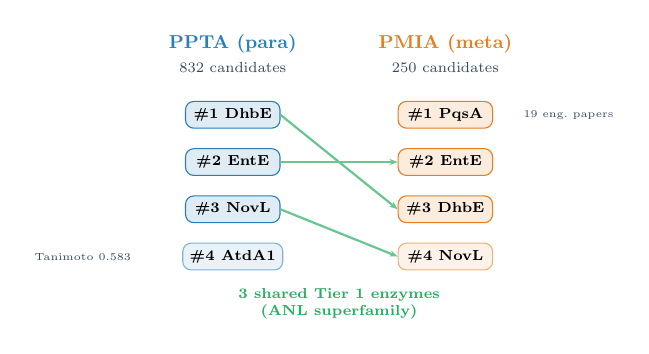
\begin{tikzpicture}[scale=0.75, transform shape,
    enzyme/.style={rectangle, rounded corners=3pt, minimum width=1.6cm, minimum height=0.45cm, font=\scriptsize\bfseries, text centered, draw},
]
% Headers
\node[font=\small\bfseries\color{accentblue}] at (-1.8, 3.8) {PPTA (para)};
\node[font=\small\bfseries\color{accentorange}] at (1.8, 3.8) {PMIA (meta)};
\node[font=\scriptsize\color{darkgray}] at (-1.8, 3.4) {832 candidates};
\node[font=\scriptsize\color{darkgray}] at (1.8, 3.4) {250 candidates};

% PPTA ranks (left)
\node[enzyme, fill=accentblue!15, draw=accentblue] (p1) at (-1.8, 2.6) {\#1 DhbE};
\node[enzyme, fill=accentblue!15, draw=accentblue] (p2) at (-1.8, 1.8) {\#2 EntE};
\node[enzyme, fill=accentblue!15, draw=accentblue] (p3) at (-1.8, 1.0) {\#3 NovL};
\node[enzyme, fill=accentblue!10, draw=accentblue!60] (p4) at (-1.8, 0.2) {\#4 AtdA1};

% PMIA ranks (right)
\node[enzyme, fill=accentorange!15, draw=accentorange] (m1) at (1.8, 2.6) {\#1 PqsA};
\node[enzyme, fill=accentorange!15, draw=accentorange] (m2) at (1.8, 1.8) {\#2 EntE};
\node[enzyme, fill=accentorange!15, draw=accentorange] (m3) at (1.8, 1.0) {\#3 DhbE};
\node[enzyme, fill=accentorange!10, draw=accentorange!60] (m4) at (1.8, 0.2) {\#4 NovL};

% Connection lines for shared enzymes
\draw[thick, color=accentgreen!70, -{Stealth[length=3pt]}] (p1.east) -- (m3.west) node[midway, above, font=\tiny\color{accentgreen!80}] {};
\draw[thick, color=accentgreen!70, -{Stealth[length=3pt]}] (p2.east) -- (m2.west);
\draw[thick, color=accentgreen!70, -{Stealth[length=3pt]}] (p3.east) -- (m4.west);

% Unique labels
\node[font=\tiny\color{darkgray}, anchor=west] at (3.0, 2.6) {19 eng.\ papers};
\node[font=\tiny\color{darkgray}, anchor=east] at (-3.4, 0.2) {Tanimoto 0.583};

% Shared label
\node[font=\scriptsize\bfseries\color{accentgreen}, align=center] at (0, -0.6) {3 shared Tier 1 enzymes\\(ANL superfamily)};

\end{tikzpicture}
\end{center}

\end{column}
\begin{column}{0.52\textwidth}

{\scriptsize
\begin{adjustbox}{max width=\textwidth}
\begin{tabular}{@{}l l l c c@{}}
\toprule
\textbf{Gene} & \textbf{Family} & \textbf{Evidence} & \textbf{PPTA} & \textbf{PMIA}\\
\midrule
\texttt{dhbE} & Aryl-AMP & 3 PDB, 4 char. & \textbf{1} & 3\\
\texttt{entE} & Aryl-AMP & 6 PDB, 16 char. & 2 & 2\\
\texttt{novL} & Aminocoumarin & EC 6.3.1.15 & 3 & 4\\
\texttt{atdA1} & Gln syn.\ fold & 3 eng. & 4 & ---\\
\texttt{pqsA} & Anthr.-CoA & 4 PDB, 28 char. & --- & \textbf{1}\\
\bottomrule
\end{tabular}
\end{adjustbox}
}

\vspace{6pt}
\begin{exampleblock}{\scriptsize Why Rankings Differ}
\vspace{-2pt}
\begin{itemize}\scriptsize
\setlength\itemsep{1pt}
\item \textbf{PPTA}: DhbE \#1 --- direct evidence of PPD amide formation (PMID 27731335)
\item \textbf{PMIA}: PqsA \#1 --- anthranilate has dual amine/acid functionality; 19 eng.\ papers
\item Meta-substituted benzoate ligases more abundant in nature
\end{itemize}
\end{exampleblock}
\end{column}
\end{columns}
\end{frame}

% ════════════════════════════════════════════════════════════
% SLIDE 12b: Runs 3 & 4 — Native Reaction Comparison
% ════════════════════════════════════════════════════════════
\begin{frame}{Runs 3 \& 4: Native Reactions of Top Candidates}
\vspace{-6pt}

{\scriptsize
\begin{adjustbox}{max width=\textwidth}
\begin{tabular}{@{}r p{5.5cm} p{3.5cm} l@{}}
\toprule
 & \textbf{Native Reaction} & \textbf{Why Analogous} & \textbf{Evidence} \\
\midrule
\rowcolor{accentred!8}
\textbf{Target} & Ar--COOH + H\textsubscript{2}N--Ar' $\xrightarrow{\text{ATP}}$ Ar--CO--NH--Ar' & TPA/IPA + PPD/MPD $\rightarrow$ polyamide & --- \\[3pt]
\rowcolor{accentblue!8}
\textbf{DhbE} & 2,3-DHB $\xrightarrow{\text{ATP}}$ DHB-AMP $\xrightarrow{\text{PPD}}$ amide & \textbf{Proven}: forms amide with PPD & 3 PDB \\[3pt]
\rowcolor{accentorange!8}
\textbf{PqsA} & Anthranilate + CoA $\xrightarrow{\text{ATP}}$ anthraniloyl-CoA & --NH\textsubscript{2} + --COOH on same ring & 4 PDB, 28 papers \\[3pt]
\rowcolor{accentgreen!8}
\textbf{NovL} & Ar--COOH + Ar'--NH\textsubscript{2} $\xrightarrow{\text{ATP}}$ Ar--CO--NH--Ar' & \textbf{Only} native Ar--CO--NH--Ar ligase & 1 paper, AF only \\
\bottomrule
\end{tabular}
\end{adjustbox}
}

\vspace{4pt}
\begin{columns}[T]
\begin{column}{0.32\textwidth}
\begin{block}{\scriptsize DhbE / EntE (ANL superfamily)}
\vspace{-2pt}
\begin{itemize}\scriptsize
\setlength\itemsep{0pt}
\item Aryl-AMP ligase: adenylates aromatic acid, then amine attacks
\item MW 2,3-DHB (153) $\approx$ TPA/IPA (166)
\item DhbE directly forms amide with PPD (PMID 27731335)
\end{itemize}
\end{block}
\end{column}
\begin{column}{0.32\textwidth}
\begin{block}{\scriptsize PqsA (Anthranilate-CoA ligase)}
\vspace{-2pt}
\begin{itemize}\scriptsize
\setlength\itemsep{0pt}
\item Anthranilate has \textit{both} --NH\textsubscript{2} and --COOH $\approx$ MPD + IPA combined
\item 19 engineering papers, broad scope
\item Limitation: CoA thioester $\neq$ amide
\end{itemize}
\end{block}
\end{column}
\begin{column}{0.32\textwidth}
\begin{block}{\scriptsize NovL (Aminocoumarin syn.)}
\vspace{-2pt}
\begin{itemize}\scriptsize
\setlength\itemsep{0pt}
\item \textbf{Mechanistically identical}: Ar--COOH + Ar--NH\textsubscript{2} $\rightarrow$ amide in one ATP step
\item No CoA/ACP intermediate
\item Under-characterized (1 paper)
\end{itemize}
\end{block}
\end{column}
\end{columns}
\end{frame}

% ════════════════════════════════════════════════════════════
% SLIDE 13: Cross-Run Insights
% ════════════════════════════════════════════════════════════
\begin{frame}{Cross-Run Insights}
\vspace{-8pt}

\begin{columns}[T]
\begin{column}{0.42\textwidth}

\begin{center}
\includegraphics[width=\textwidth]{figs/cross_run_map.pdf}
\end{center}

\vspace{-2pt}
\begin{exampleblock}{\scriptsize Agent Adaptability}
\vspace{-2pt}
\begin{itemize}\scriptsize
\setlength\itemsep{0pt}
\item Same 18 tools, same prompts
\item Emergent search strategies per query
\item No hardcoded pathways or enzyme lists
\end{itemize}
\end{exampleblock}

\end{column}

\begin{column}{0.55\textwidth}
\begin{alertblock}{\small Top Candidate per Reaction Class}
\vspace{-2pt}
\begin{itemize}\scriptsize
\setlength\itemsep{2pt}
\item \textbf{Aliphatic} --- \texttt{asbA}/\texttt{asbB}: documented diacid--diamine promiscuity; K313A/M mutants accept C8 diamines
\item \textbf{Hydrolysis} --- \texttt{nylC}: confirmed nylon-66 activity; 11 PDB, 9 eng.
\item \textbf{Para-aromatic} --- \texttt{dhbE}: direct evidence of PPD amide formation
\item \textbf{Meta-aromatic} --- \texttt{pqsA}: 4 PDB, 19 eng.; anthranilate (dual amine/acid)
\item \textbf{Outlier} --- \texttt{novL}: only native ArCO--NH--Ar amide ligase
\end{itemize}
\end{alertblock}
\end{column}
\end{columns}
\end{frame}

% ════════════════════════════════════════════════════════════
% ════════════════════════════════════════════════════════════
% SLIDE 13b: Enzyme Family Landscape + Tool Usage
% ════════════════════════════════════════════════════════════
\begin{frame}{Enzyme Families and Tool Usage Across Runs}
\vspace{-8pt}

\begin{columns}[T]
\begin{column}{0.50\textwidth}
\begin{center}
\includegraphics[width=\textwidth]{figs/family_landscape.pdf}
\end{center}
\end{column}
\begin{column}{0.50\textwidth}
\begin{center}
\includegraphics[width=\textwidth]{figs/tool_usage.pdf}
\end{center}
\end{column}
\end{columns}

\vspace{-2pt}
\begin{center}
\colorbox{lightblue!40}{\parbox{0.92\textwidth}{\centering\scriptsize
\textbf{Left:} Bubble size $\propto$ candidates evaluated per family. No family overlap between aliphatic and aromatic runs.
\textbf{Right:} Database search dominates (47\%), followed by evaluation (30\%) and literature (20\%).
}}
\end{center}
\end{frame}

% ════════════════════════════════════════════════════════════
% SLIDE 13c: Example Report Excerpt
% ════════════════════════════════════════════════════════════
\begin{frame}{Example: Agent-Generated Candidate Table (Run 3, PPTA)}
\vspace{-6pt}
\begin{center}
\includegraphics[width=0.82\textwidth]{figs/report_excerpt.pdf}
\end{center}

\vspace{-4pt}
\begin{columns}[T]
\begin{column}{0.48\textwidth}
\begin{block}{\scriptsize Report Contents}
\vspace{-2pt}
\begin{itemize}\scriptsize
\setlength\itemsep{0pt}
\item Executive summary with reaction analysis
\item Candidate table with hyperlinked IDs
\item Top candidate profiles with native reactions
\item Key references with PMIDs
\end{itemize}
\end{block}
\end{column}
\begin{column}{0.48\textwidth}
\begin{alertblock}{\scriptsize Dual Ranking}
\vspace{-2pt}
\begin{itemize}\scriptsize
\setlength\itemsep{0pt}
\item \textbf{Report 1}: ranks by evidence (Swiss-Prot, PDB, mutagenesis)
\item \textbf{Report 2}: ranks by substrate match
\item Both auto-generated per run
\end{itemize}
\end{alertblock}
\end{column}
\end{columns}
\end{frame}

% ════════════════════════════════════════════════════════════
% SLIDE 14: Conclusions
% ════════════════════════════════════════════════════════════
{
\setbeamercolor{background canvas}{bg=deepblue}
\begin{frame}[plain]
\vfill
\begin{center}
{\Large\bfseries\color{white} Conclusions}\\[12pt]
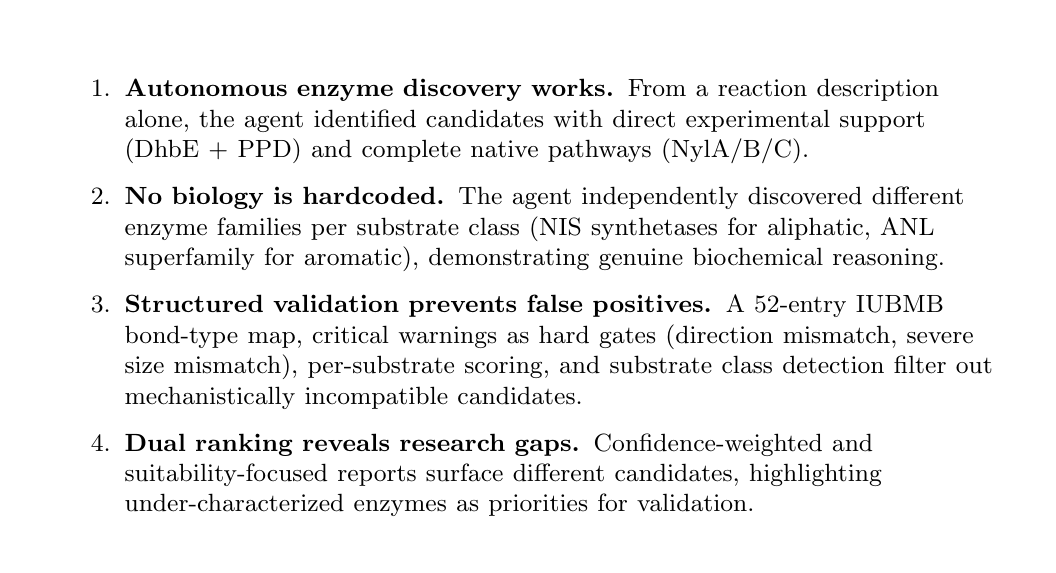
\begin{tikzpicture}
\node[rectangle, rounded corners=8pt, fill=white, text width=12cm, inner sep=10pt, align=left] {
\small
\begin{enumerate}\setlength\itemsep{4pt}
\item \textbf{Autonomous enzyme discovery works.} From a reaction description alone, the agent identified candidates with direct experimental support (DhbE + PPD) and complete native pathways (NylA/B/C).

\item \textbf{No biology is hardcoded.} The agent independently discovered different enzyme families per substrate class (NIS synthetases for aliphatic, ANL superfamily for aromatic), demonstrating genuine biochemical reasoning.

\item \textbf{Structured validation prevents false positives.} A 52-entry IUBMB bond-type map, critical warnings as hard gates (direction mismatch, severe size mismatch), per-substrate scoring, and substrate class detection filter out mechanistically incompatible candidates.

\item \textbf{Dual ranking reveals research gaps.} Confidence-weighted and suitability-focused reports surface different candidates, highlighting under-characterized enzymes as priorities for validation.
\end{enumerate}
};
\end{tikzpicture}
\end{center}
\vfill
\end{frame}
}

% ════════════════════════════════════════════════════════════
% APPENDIX
% ════════════════════════════════════════════════════════════
{
\setbeamercolor{background canvas}{bg=deepblue}
\begin{frame}[plain]
\vfill
\begin{center}
{\Large\bfseries\color{white} Appendix}\\[10pt]
{\large\color{lightblue!80} Technical Details}
\end{center}
\vfill
\end{frame}
}

% ── A1: 7 Discovery Principles ────────────────────────────
\begin{frame}{Appendix A1: Discovery Principles (P1--P7)}
\vspace{-6pt}
{\scriptsize
\begin{tabular}{@{}c l p{9.5cm}@{}}
\toprule
 & \textbf{Principle} & \textbf{Description} \\
\midrule
\textbf{P1} & Decompose before searching & Analyze target bond type, mechanism, and substrate properties \textit{before} any database query \\
\textbf{P2} & Build understanding iteratively & Start with reviews; follow citation networks to discover specific enzymes \\
\textbf{P3} & Search broadly (6 axes) & EC numbers, substrate analogues, bond type keywords, pathway names, gene names, InterPro domains --- EC-only searches \textit{will} miss entire families \\
\textbf{P4} & Evaluate with chemical reasoning & Reason about mechanism, substrate size/shape/chemistry --- not just scores \\
\textbf{P5} & Structural analysis when it adds value & Distinguish similar candidates; assess substrate fit in active site \\
\textbf{P6} & Persist your reasoning & Record analysis, decisions, gaps in research notebook to prevent context loss \\
\textbf{P7} & Reflect periodically & Every $\sim$5 iterations: review progress, identify gaps, change strategy if needed \\
\bottomrule
\end{tabular}
}
\vspace{4pt}
\begin{center}
\colorbox{lightblue!50}{\parbox{0.88\textwidth}{\centering
\scriptsize Principles are \textbf{generic} --- no hardcoded enzyme names, substrates, or pathways. All discovery emerges from LLM reasoning guided by these principles.
}}
\end{center}
\end{frame}

% ── A2: Phase 1 Detail — Reaction Analysis ─────────────────
\begin{frame}{Appendix A2: Phase 1 --- Reaction Analysis (Most Critical Phase)}
\vspace{-4pt}
\begin{columns}[T]
\begin{column}{0.48\textwidth}
\begin{block}{\small Step A: Substrate Analysis}
\vspace{-2pt}
\begin{itemize}\scriptsize
\setlength\itemsep{0pt}
\item Classify target bond type and reaction direction
\item Analyze substrate functional groups, size, reactivity
\item Identify natural metabolites resembling each substrate
\end{itemize}
\end{block}

\begin{block}{\small Step B: Mechanism Enumeration}
\vspace{-2pt}
\begin{itemize}\scriptsize
\setlength\itemsep{0pt}
\item Identify $\geq$3 distinct enzymatic mechanisms
\item Each must have different activated intermediate and protein fold
\item Name mechanism, fold/domain family, EC sub-class
\end{itemize}
\end{block}
\end{column}
\begin{column}{0.48\textwidth}
\begin{alertblock}{\small Step C: Molecule Enumeration (Critical)}
\vspace{-2pt}
\begin{itemize}\scriptsize
\setlength\itemsep{0pt}
\item List \textbf{ALL} molecules in biology containing target bond type
\item Search exhaustively: amino acid derivatives, cofactors, cell wall components, siderophores, antibiotics, biopolymers, PTMs, signaling molecules
\item Aim for \textbf{20+ molecules} total
\item Each molecule name $\rightarrow$ search term
\end{itemize}
\end{alertblock}

\begin{exampleblock}{\small Step D: Search Specification}
\vspace{-2pt}
\begin{itemize}\scriptsize
\setlength\itemsep{0pt}
\item Write search plan \textit{before} any search tool call
\item ec\_prefixes, keywords, literature\_terms (8--12 diverse)
\item Every enzyme name $\rightarrow$ individual UniProt search
\end{itemize}
\end{exampleblock}
\end{column}
\end{columns}
\end{frame}

% ── A3: Search Strategy Details ─────────────────────────────
\begin{frame}{Appendix A3: Multi-Axis Search Strategy}
\vspace{-4pt}
\begin{columns}[T]
\begin{column}{0.48\textwidth}
\begin{block}{\small 6 Search Axes}
\vspace{-2pt}
\begin{itemize}\scriptsize
\setlength\itemsep{1pt}
\item \textbf{EC numbers}: complete + partial prefixes (e.g., 6.3, 6.3.2)
\item \textbf{Substrate analogues}: structural similarity to target
\item \textbf{Bond type keywords}: reaction mechanism terms
\item \textbf{Pathway names}: natural products containing target bond
\item \textbf{Gene names}: extracted from literature abstracts
\item \textbf{InterPro domains}: protein fold/family identifiers
\end{itemize}
\end{block}

\begin{alertblock}{\small Query Construction Rules}
\vspace{-2pt}
\begin{itemize}\scriptsize
\setlength\itemsep{0pt}
\item PubMed queries: \textbf{3--5 words} with \texttt{[Title/Abstract]}
\item Queries $>$8 words $\rightarrow$ almost always return 0 results
\item Search each gene name \textbf{individually} (never OR-joined)
\item Short gene names ($\leq$4 chars): add \texttt{function\_filter}
\end{itemize}
\end{alertblock}
\end{column}
\begin{column}{0.48\textwidth}
\begin{exampleblock}{\small Exhaustive Coverage Checklist}
\vspace{-2pt}
\begin{itemize}\scriptsize
\setlength\itemsep{1pt}
\item Primary metabolism (amino acids, cofactors)
\item Cell wall / membrane biosynthesis
\item Secondary metabolites (antibiotics, siderophores, toxins)
\item Storage compounds and biopolymers
\item Post-translational modifications
\item Xenobiotic metabolism
\end{itemize}
\vspace{2pt}
{\tiny\color{accentred} For each context: identify specific enzymes, search individually}
\end{exampleblock}

\begin{block}{\small Literature Mining}
\vspace{-2pt}
\begin{itemize}\scriptsize
\setlength\itemsep{0pt}
\item Abstracts often lack gene names --- those are in full text
\item \texttt{deep\_literature\_search}: follow citation networks
\item \texttt{extract\_entities}: NLP-based gene/EC extraction
\item Semantic re-ranking (nomic-embed-text-v1.5, cosine sim $\geq$0.25)
\end{itemize}
\end{block}
\end{column}
\end{columns}
\end{frame}

% ── A4: Bond-Type Classification ─────────────────────────────
\begin{frame}{Appendix A4: IUBMB Bond-Type Classification System}
\vspace{-8pt}
\begin{columns}[T]
\begin{column}{0.48\textwidth}
\begin{block}{\small EC $\rightarrow$ Bond-Type Map (72 entries)}
\vspace{-2pt}
{\scriptsize
\begin{tabular}{@{}l c l l@{}}
\toprule
\textbf{EC Class} & \textbf{N} & \textbf{Direction} & \textbf{Example} \\
\midrule
1 Oxidoreductases & 17 & redox & C-OH, C=O, C-N \\
2 Transferases & 10 & transfer & acyl, amino, phospho \\
3 Hydrolases & 13 & cleavage & ester, peptide, amide \\
4 Lyases & 7 & cleavage & C-C, C-O, C-N \\
5 Isomerases & 7 & isomzn. & cis/trans, stereo \\
6 Ligases & 6 & formation & ester, amide, C-C \\
7 Translocases & 6 & translcn. & various coupling \\
\midrule
& \textbf{66} & & \\
\bottomrule
\end{tabular}
}
\end{block}

\begin{block}{\small Reaction-Text Heuristics}
\vspace{-2pt}
\begin{itemize}\scriptsize
\setlength\itemsep{0pt}
\item CoA in reaction $\rightarrow$ thioester
\item \texttt{[ACP]}, \texttt{[ArCP]}, \texttt{holo-[...]} $\rightarrow$ carrier-tethered
\item NH\textsubscript{4}\textsuperscript{+}, ammonia $\rightarrow$ primary amide indicator
\end{itemize}
\end{block}
\end{column}
\begin{column}{0.48\textwidth}
\begin{alertblock}{\small Mismatch Detection Logic}
\vspace{-2pt}
\begin{itemize}\scriptsize
\setlength\itemsep{1pt}
\item \textbf{Bond-type equivalence}: amide $\approx$ C-N (expanded sets)
\item \textbf{Bond-type mismatch}: no intersection between enzyme and target bond types $\rightarrow$ \textbf{CRITICAL}
\item \textbf{Direction mismatch}: formation $\leftrightarrow$ cleavage is a hard conflict $\rightarrow$ \textbf{CRITICAL}
\item \textbf{Peptide vs.\ amide}: EC 3.4 (peptide hydrolase) on non-peptide target $\rightarrow$ substrate class warning
\end{itemize}
\end{alertblock}

\begin{exampleblock}{\small Target Reaction Parsing}
\vspace{-2pt}
{\tiny 14 bond-type keywords: thioester, phospho(di)ester, glycosidic, disulfide, peptide, amide, ester, ether, C-C/N/O/S}

\vspace{1pt}
\begin{itemize}\scriptsize
\setlength\itemsep{-1pt}
\item Formation: synthesis, ligation, condensation, ligase
\item Cleavage: hydrolysis, degradation, decarboxylation
\item Transfer: phosphorylation, glycosylation, acylation
\end{itemize}
\end{exampleblock}
\end{column}
\end{columns}
\end{frame}

% ── A5: Substrate Similarity Pipeline ────────────────────────
\begin{frame}{Appendix A5: Substrate Similarity Pipeline}
\vspace{-8pt}
\begin{columns}[T]
\begin{column}{0.48\textwidth}
\begin{block}{\small Resolution \& Fingerprint}
\vspace{-2pt}
\begin{itemize}\scriptsize
\setlength\itemsep{0pt}
\item Catalytic activity $\rightarrow$ ChEBI IDs $\rightarrow$ SMILES (OLS4 API, cached)
\item 17 cofactors excluded (H\textsubscript{2}O, ATP/ADP/AMP, CoA, NAD\textsuperscript{+}/NADH, \ldots)
\item ECFP4 fingerprint (radius=2, 2048 bits), Tanimoto $\in [0,1]$
\item Multi-substrate: geometric mean (floor $10^{-6}$)
\end{itemize}
\end{block}

\begin{alertblock}{\small Ranking Priority}
\vspace{-2pt}
\begin{itemize}\scriptsize
\setlength\itemsep{-1pt}
\item \textbf{Primary}: FG \textit{counts} (carboxyl, amine, hydroxyl, thiol)
\item \textbf{Secondary}: MW similarity, chain length
\item \textbf{Reference}: Tanimoto (unreliable for non-natural targets)
\end{itemize}
\end{alertblock}
\end{column}
\begin{column}{0.48\textwidth}
\begin{exampleblock}{\small Property-Based Comparison (12 metrics)}
\vspace{-2pt}
{\tiny
\begin{tabular}{@{}l l | l l@{}}
\toprule
\textbf{Property} & \textbf{Algorithm} & \textbf{Property} & \textbf{Algorithm} \\
\midrule
MW similarity & min/max ratio & FG Jaccard & $|A \cap B| / |A \cup B|$ \\
Volume similarity & min/max ratio & H-bond donors & $|\Delta|$ \\
Chain length & $1 - |\Delta| / \max$ & H-bond acceptors & $|\Delta|$ \\
LogP similarity & $1 - |\Delta| / 5.0$ & Rotatable bonds & $|\Delta|$ \\
TPSA similarity & min/max ratio & Aromaticity & match (bool) \\
Net charge pH\,8 & comparison & Cyclicity & match (bool) \\
\bottomrule
\end{tabular}
}
\end{exampleblock}

\begin{block}{\small One-Sided Mismatch Detection}
\vspace{-2pt}
\begin{itemize}\scriptsize
\setlength\itemsep{0pt}
\item Multi-substrate: best/bottleneck ratio $>$ 3$\times$ $\rightarrow$ warning
\item Prevents one good match masking a poor match on another substrate
\end{itemize}
\end{block}
\end{column}
\end{columns}
\end{frame}

% ── A6: Strengths & Weaknesses Detection ─────────────────────
\begin{frame}{Appendix A6: Automated Strengths \& Weaknesses}
\vspace{-8pt}
\begin{columns}[T]
\begin{column}{0.48\textwidth}
\begin{exampleblock}{\small Strengths (Informational)}
\vspace{-2pt}
{\scriptsize
\begin{tabular}{@{}p{4.2cm} l@{}}
\toprule
\textbf{Condition} & \textbf{Threshold} \\
\midrule
Swiss-Prot reviewed & boolean \\
Strong EC match & depth $\geq$ 3 \\
Well-characterized & $\geq$5 char.\ papers \\
Engineering precedent & $\geq$2 eng.\ papers \\
Mutagenesis data & $>$0 variants \\
Crystal structure & $>$0 PDB IDs \\
AlphaFold available & boolean \\
\bottomrule
\end{tabular}
}
\end{exampleblock}

\begin{block}{\small Substrate Classification}
\vspace{-2pt}
\begin{itemize}\scriptsize
\setlength\itemsep{-1pt}
\item \textbf{polymer}: \texttt{(n)}, \texttt{poly[-(]}, NRPS/PKS
\item \textbf{carrier\_tethered}: ACP, ArCP, pantetheine
\item \texttt{required\_cofactors}: from UniProt COFACTOR
\end{itemize}
\end{block}
\end{column}
\begin{column}{0.48\textwidth}
\begin{alertblock}{\small Critical Warnings (Hard Gates)}
\vspace{-2pt}
{\scriptsize
\begin{tabular}{@{}p{3.5cm} l@{}}
\toprule
\textbf{Condition} & \textbf{Threshold} \\
\midrule
Bond-type mismatch & no intersection \\
Direction mismatch & formation $\leftrightarrow$ cleavage \\
Severe size mismatch & MW sim $<$ 0.15 \\
\bottomrule
\end{tabular}
}
\vspace{2pt}
{\tiny\color{accentred} Require specific PMID to override. LLM cannot dismiss.}
\end{alertblock}

\begin{block}{\small Regular Weaknesses}
\vspace{-2pt}
{\scriptsize
\begin{tabular}{@{}p{3.5cm} l@{}}
\toprule
\textbf{Condition} & \textbf{Threshold} \\
\midrule
Moderate size mismatch & MW sim $<$ 0.30 \\
One-sided mismatch & ratio $>$ 3$\times$ \\
Peptide/amide class note & EC 3.4 on non-peptide \\
Polymer substrate & regex match \\
TrEMBL (unreviewed) & boolean \\
No EC match & no target overlap \\
No char.\ papers & 0 papers \\
No structural data & no PDB/AF \\
\bottomrule
\end{tabular}
}
\end{block}
\end{column}
\end{columns}
\end{frame}

% ── A7: Anti-Patterns ────────────────────────────────────────
\begin{frame}{Appendix A7: Anti-Patterns (Embedded in System Prompt)}
\vspace{-8pt}
\begin{columns}[T]
\begin{column}{0.48\textwidth}
\begin{alertblock}{\small Search Anti-Patterns}
\vspace{-2pt}
\begin{itemize}\scriptsize
\setlength\itemsep{1pt}
\item Do NOT search \textbf{only by EC number} --- many enzymes lack complete EC
\item Do NOT \textbf{stop after a handful} of candidates --- verify ALL contexts
\item Do NOT \textbf{repeat same search} with minor wording (deduplication catches this)
\item Do NOT use \textbf{long PubMed queries} ($>$8 words return 0 results)
\item Do NOT \textbf{skip families} from reaction analysis --- every mechanism and natural product must have a search
\item Do NOT \textbf{pivot to evaluation} until all families searched
\end{itemize}
\end{alertblock}
\end{column}
\begin{column}{0.48\textwidth}
\begin{block}{\small Evaluation Anti-Patterns}
\vspace{-2pt}
\begin{itemize}\scriptsize
\setlength\itemsep{1pt}
\item Do NOT generate a report \textbf{without evaluating} all promising candidates
\item Do NOT include enzymes whose native reaction is the \textbf{REVERSE} of the target
\item Do NOT \textbf{stop early} without completing evaluation and ranking
\item Do NOT \textbf{dump raw data} into notebook --- write synthesized analysis
\item Do NOT \textbf{ask user} for permission --- agent is fully autonomous
\end{itemize}
\end{block}

\vspace{2pt}
\begin{exampleblock}{\small Coverage Enforcement}
\vspace{-2pt}
\begin{itemize}\scriptsize
\setlength\itemsep{0pt}
\item Reflection checkpoint every 5 iterations
\item Warning if $<$15 candidates from $<$5 families
\item Agent must verify every family has candidates
\end{itemize}
\end{exampleblock}
\end{column}
\end{columns}
\end{frame}

% ── A8: Context Management ──────────────────────────────────
\begin{frame}{Appendix A8: Context Management \& Artifact System}
\vspace{-8pt}
\begin{columns}[T]
\begin{column}{0.48\textwidth}
\begin{block}{\small LLM Context Compaction (\texttt{\_compact\_for\_llm})}
\vspace{-2pt}
{\scriptsize
\begin{tabular}{@{}l l l@{}}
\toprule
\textbf{Strategy} & \textbf{Keys} & \textbf{Limit} \\
\midrule
Strip & sequence, openalex\_id & removed \\
Truncate & abstract & 200 chars \\
 & description & 200 chars \\
Cap list & papers & 8 items \\
 & results, entries, hits & 10 items \\
 & genes & 3 items \\
 & authors & 3 items \\
 & catalytic\_activities & 3 items \\
\bottomrule
\end{tabular}
}
\vspace{2pt}
{\tiny Full data always preserved in \texttt{artifacts/} directory}
\end{block}

\begin{block}{\small Search Deduplication}
\vspace{-2pt}
\begin{itemize}\scriptsize
\setlength\itemsep{0pt}
\item Similarity = max(Jaccard\textsubscript{tokens}, SequenceMatcher\textsubscript{chars})
\item Threshold: $\geq$0.90 $\rightarrow$ return cached result
\item Applies to literature + database search tools
\end{itemize}
\end{block}
\end{column}
\begin{column}{0.48\textwidth}
\begin{exampleblock}{\small Artifact File Structure}
\vspace{-2pt}
{\tiny
\begin{verbatim}
run_dir/
  artifacts/
    literature/*.json
    database/*.json
    candidates/*.json
  agent_state/messages.json
  notebook.json
  candidate_registry.json
  exploration_log.md
  report_confidence.md
  report_explorative.md
  candidates.csv
  top_candidates/*.pdb
  token_usage.json
\end{verbatim}
}
\end{exampleblock}
\end{column}
\end{columns}
\end{frame}

% ── A9: Dual Report System ──────────────────────────────────
\begin{frame}{Appendix A9: Dual Report Generation}
\vspace{-4pt}
\begin{columns}[T]
\begin{column}{0.48\textwidth}
\begin{block}{\small Confidence-Weighted Report}
\vspace{-2pt}
\begin{itemize}\scriptsize
\setlength\itemsep{1pt}
\item \textbf{Ranking}: experimental evidence drives position
\item Sections: Executive Summary, Enzyme Families, Candidate Table, Tier 1 Profiles, Key References, Mechanistic Summary
\item Consolidate orthologs; hyperlink UniProt IDs and PMIDs
\item Excludes: experimental strategy, risk assessment, cofactor SMILES
\end{itemize}
\end{block}

\begin{block}{\small Generation Flow}
\vspace{-2pt}
\begin{itemize}\scriptsize
\setlength\itemsep{0pt}
\item \textbf{In-run}: LLM generates confidence report when it stops calling tools
\item \textbf{Rerank prompt}: injected to generate explorative report
\item \textbf{Fallback}: post-hoc LLM call if in-run times out
\item Temperature: 0.2 (confidence), 0.3 (explorative)
\end{itemize}
\end{block}
\end{column}
\begin{column}{0.48\textwidth}
\begin{alertblock}{\small Suitability-Focused (Explorative) Report}
\vspace{-2pt}
\begin{itemize}\scriptsize
\setlength\itemsep{1pt}
\item \textbf{Ranking}: biochemical suitability drives position
\item Evidence $\rightarrow$ separate \textbf{Confidence column} (High/Medium/Low/Minimal) that does \textbf{NOT} affect rank
\item Same candidate table format + comparison note
\end{itemize}
\end{alertblock}

\vspace{2pt}
\begin{exampleblock}{\small Confidence Level Assignment}
\vspace{-2pt}
{\scriptsize
\begin{tabular}{@{}l p{4.5cm}@{}}
\toprule
\textbf{Level} & \textbf{Criteria} \\
\midrule
High & Swiss-Prot + $\geq$5 char.\ + crystal structure \\
Medium & Swiss-Prot OR $\geq$2 char.\ OR eng.\ precedent \\
Low & TrEMBL + $\leq$1 paper + AlphaFold only \\
Minimal & No characterization, no EC, predicted only \\
\bottomrule
\end{tabular}
}
\end{exampleblock}
\end{column}
\end{columns}
\end{frame}

% ── A10: Configuration Thresholds ────────────────────────────
\begin{frame}{Appendix A10: Configuration Parameters}
\vspace{-6pt}
\begin{columns}[T]
\begin{column}{0.48\textwidth}
{\scriptsize
\begin{tabular}{@{}l r p{3.2cm}@{}}
\toprule
\textbf{Parameter} & \textbf{Value} & \textbf{Purpose} \\
\midrule
\multicolumn{3}{@{}l}{\textit{Agent Control}} \\
MAX\_ITERATIONS & 30 & Agent loop limit \\
REFLECTION\_INTERVAL & 5 & Reflection frequency \\
LLM\_TIMEOUT & 120\,s & Per-call timeout \\
LLM\_TEMPERATURE & 0.2 & Discovery/eval \\
EXPL\_REPORT\_TEMP & 0.3 & Explorative report \\
\midrule
\multicolumn{3}{@{}l}{\textit{Tool Execution}} \\
THREAD\_POOL\_WORKERS & 4 & Parallel execution \\
MAX\_RESULT\_CHARS & 20{,}000 & Result truncation \\
OVERFETCH\_RATIO & 3 & Re-rank buffer \\
RERANK\_MIN\_SCORE & 0.25 & Semantic threshold \\
SCREENING\_BATCH & 10 & Screen batch size \\
\bottomrule
\end{tabular}
}
\end{column}
\begin{column}{0.48\textwidth}
{\scriptsize
\begin{tabular}{@{}l r p{3.2cm}@{}}
\toprule
\textbf{Parameter} & \textbf{Value} & \textbf{Purpose} \\
\midrule
\multicolumn{3}{@{}l}{\textit{Evaluation Thresholds}} \\
EC\_MATCH\_STRONG & 3 & Depth for strength \\
MW\_SEVERE & 0.15 & $\sim$6.7$\times$ ratio \\
MW\_MODERATE & 0.30 & $\sim$3.3$\times$ ratio \\
WELL\_CHAR\_THRESH & 5 & Min char.\ papers \\
ENG\_PRECEDENT & 2 & Min eng.\ papers \\
ENG\_PAPER\_WEIGHT & 2 & Scoring multiplier \\
GEOM\_MEAN\_FLOOR & $10^{-6}$ & Multi-substrate \\
\midrule
\multicolumn{3}{@{}l}{\textit{Database Limits}} \\
UNIPROT\_MAX & 500 & Results cap \\
KEGG\_EC\_LIMIT & 25 & Per-EC cap \\
INTERPRO\_PAGE & 50 & Page size cap \\
\bottomrule
\end{tabular}
}
\end{column}
\end{columns}
\end{frame}

\end{document}
